% $Id$ %
\appendix

% $Id$ %
\chapter{File formats}
\section{\label{ref:Supportedfileformats}Supported file formats}
\begin{rbtabular}{\textwidth}{cl>{\raggedright}p{7em}X}%
{\textbf{Icon} & \textbf{File Type} & \textbf{Extension} 
  & \textbf{Action when selected}}{}{}

\includegraphics[width=0.37cm]{appendix/images/icon-directory.png} 
  & Directory & \emph{none} & Enter the directory \tabularnewline
\opt{recorder,recorderv2fm,ondiofm,ondiosp}{
  
\includegraphics[width=0.37cm]{appendix/images/icon-rolo.png} 
  & Rockbox firmware & \fname{.ajz} & Load the new firmware with ROLO \tabularnewline
}
\opt{swcodec}{
  
\includegraphics[width=0.37cm]{appendix/images/icon-audio-file.png} 
  & Audio file & \emph{various}\newline%
  (see \ref{ref:Supportedaudioformats})%
  % do NOT use \reference{} here as that will break the table.
  & Start playing the file and show the WPS\tabularnewline
}
  & Bookmark & \fname{.bmark} & Display all bookmarks for an audio file\tabularnewline
\opt{lcd_bitmap}{
  & Game of Life & \fname{.cells} & Show the configuration with the
     ``Rocklife'' plugin\tabularnewline
}

\includegraphics[width=0.37cm]{appendix/images/icon-config.png} 
  & Configuration File & \fname{.cfg} & Load the settings file\tabularnewline

\includegraphics[width=0.37cm]{appendix/images/icon-chip8.png} 
  & Chip8 game & \fname{.ch8} & Play the Chip8 game \tabularnewline
\opt{lcd_color}{
  & Colours & \fname{.colours} & Open the colours file for editing.
    See \reference{ref:ChangingFiletypeColours}.\tabularnewline
}

\includegraphics[width=0.37cm]{appendix/images/icon-cuesheet.png} 
  & Cuesheet & \fname{.cue} & View the cuesheet file \tabularnewline
\opt{radio}{
  & FM Presets & \fname{.fmr} & Load the FM Presets (previous are discarded)\tabularnewline
}

\includegraphics[width=0.37cm]{appendix/images/icon-font.png} 
  & Font & \fname{.fnt} & Change the user interface font to this one\tabularnewline
\opt{gigabeat}{
  
\includegraphics[width=0.37cm]{appendix/images/icon-rolo.png} 
  & Rockbox firmware & \fname{.gigabeat} & Load the new firmware with ROLO \tabularnewline
}
\opt{iaudio}{
  
\includegraphics[width=0.37cm]{appendix/images/icon-rolo.png} 
  & Rockbox firmware & \fname{.iaudio} & Load the new firmware with ROLO \tabularnewline
}
\opt{ipod}{
  
\includegraphics[width=0.37cm]{appendix/images/icon-rolo.png} 
  & Rockbox firmware & \fname{.ipod} & Load the new firmware with ROLO \tabularnewline
}
\opt{iriverh100,iriverh300}{
  
\includegraphics[width=0.37cm]{appendix/images/icon-rolo.png} 
  & Rockbox firmware & \fname{.iriver} & Load the new firmware with ROLO \tabularnewline
}

\includegraphics[width=0.37cm]{appendix/images/icon-image-file.png} 
  & Image & \fname{.jpg} & View the JPEG image \tabularnewline
  & Link & \fname{.link} & Display list of target files and directories;
    selecting one jumps to the target. See \reference{ref:Shortcutsplugin}.\tabularnewline

\includegraphics[width=0.37cm]{appendix/images/icon-lang.png} 
  & Language File & \fname{.lng} & Load the language file \tabularnewline

\includegraphics[width=0.37cm]{appendix/images/icon-playlist.png}
  & Playlist & \fname{.m3u}, \fname{.m3u8} & Load the playlist and start playing 
    the first file \tabularnewline
\opt{iriverh10,iriverh10_5gb,sansa,vibe500}{
  
\includegraphics[width=0.37cm]{appendix/images/icon-rolo.png} 
  & Rockbox firmware & \fname{.mi4} & Load the new firmware with ROLO \tabularnewline
}
\opt{player}{
  
\includegraphics[width=0.37cm]{appendix/images/icon-rolo.png} 
  & Rockbox firmware & \fname{.mod} & Load the new firmware with ROLO \tabularnewline
}
\opt{masd,masf}{
  
\includegraphics[width=0.37cm]{appendix/images/icon-audio-file.png} 
  & Audio file & \fname{.mp2}, \fname{.mp3} & Start playing the file and show the WPS\tabularnewline
}
\opt{swcodec}{
 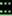
\includegraphics[width=0.37cm]{appendix/images/icon-movie-file.png}
 & Video & \fname{.mpg}, \fname{.mpeg}, \fname{.mpv}, \fname{.m2v} & Play the MPEG1/2 video \tabularnewline
}

\includegraphics[width=0.37cm]{appendix/images/icon-rock.png} 
  & Plugin & \fname{.rock} & Start the plugin\tabularnewline
\opt{masf}{\opt{lcd_bitmap}{
  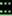
\includegraphics[width=0.37cm]{appendix/images/icon-movie-file.png} 
    & Rockbox Video & \fname{.rvf} & View the movie (Rockbox format)\tabularnewline}
}
\opt{sansaAMS}{
  
\includegraphics[width=0.37cm]{appendix/images/icon-rolo.png} 
  & Rockbox firmware & \fname{.sansa} & Load the new firmware with ROLO \tabularnewline
}

\includegraphics[width=0.37cm]{appendix/images/icon-text.png} 
  & Text File & \fname{.txt} & Display the text file using the text viewer plugin\tabularnewline
\opt{archos}{
  
\includegraphics[width=0.37cm]{appendix/images/icon-ucl.png} 
    & Flash Image & \fname{.ucl} & Flash the Rockbox image into the ROM \tabularnewline
  }
  & Voice file & \fname{.voice} & Allow Rockbox to speak menus\tabularnewline
\opt{masf}{
  
\includegraphics[width=0.37cm]{appendix/images/icon-wav-file.png} 
    & Wave Audio File & \fname{.wav} & Play the WAV file \tabularnewline%
}

\includegraphics[width=0.37cm]{appendix/images/icon-wps.png} 
  & While Playing Screen & \fname{.wps} & Load the new WPS display configuration\tabularnewline
\end{rbtabular}

\opt{swcodec}{
  \chapter{Audio and metadata formats}
  \section{\label{ref:Supportedaudioformats}Supported audio formats}
  \subsection{Lossy Codecs}
  \begin{rbtabular}{\textwidth}{l>{\raggedright}p{6em}X}%
  {\textbf{Format} & \textbf{Extension} & \textbf{Notes}}{}{}
    ATSC A/52 (AC3)
        & \fname{.a52}, \fname{.ac3}, \fname{.rm}, \fname{.ra}, \fname{.rmvb}
        & Supports downmixing for playback of 5.1 streams in stereo\\
    ADX
        & \fname{.adx} 
        & \\
    Advanced Audio Coding
        & \fname{.m4a}, \fname{.m4b}, \fname{.mp4}, \fname{.rm}, \fname{.ra}, \fname{.rmvb}
        \nopt{clipv1,c200v2}{
            & Supports AAC-LC, -HEv1, and -HEv2 profiles\\}
        \opt{clipv1,c200v2}{ % low memory targets (CODEC_SIZE <= 512 KB)
            & Supports AAC-LC profile\\}
    MPEG audio
        & \fname{.mpa}, \fname{.mp1}, \fname{.mp2}, \fname{.mp3} 
        & MPEG 1/2/2.5 Layer 1/2/3\\
    Musepack
        & \fname{.mpc} 
        & Supports SV7 and SV8 in mono/stereo \\
    OGG/Vorbis
        & \fname{.ogg}, \fname{.oga} 
        & Playback of some old ``floor 0'' files may fail on low memory targets.
          Files with album art larger than available RAM will be skipped. 
          Chained Ogg files are not supported.\\
    Sony Audio
        & \fname{.oma}, \fname{.aa3}, \fname{.rm}, \fname{.ra}, \fname{.rmvb}
        & Supports ATRAC3\\
    RealAudio
        & \fname{.rm}, \fname{.ra}, \fname{.rmvb}
        & Supports RealAudio G2 (Cook)\\
    Speex
        & \fname{.spx} 
        & \\
    Dialogic telephony type
        & \fname{.vox} 
        & \\
    Windows Media Audio Standard
        & \fname{.wma}, \fname{.wmv}, \fname{.asf} 
        & \\
    Windows Media Audio Professional
        & \fname{.wma}, \fname{.wmv}, \fname{.asf} 
        & \\
  \end{rbtabular}
  
  \note{AAC-HE profiles might not play in realtime on all devices due to CPU 
  performance requirements.}

  \subsection{Lossless Codecs}
  \begin{rbtabular}{\textwidth}{lp{6em}X}%
  {\textbf{Format} & \textbf{Extension} & \textbf{Notes}}{}{}
    Audio Interchange File Format
        & \fname{.aif}, \fname{.aiff} 
        & Linear PCM 8/16/24/32 bit, IEEE float 32/64 bit, ITU-T G.711 a-law/$\mu$-law,
          QuickTime IMA ADPCM\\
    Monkey's Audio
        & \fname{.ape}, \fname{.mac} 
        & 
        \opt{gigabeatf,iriverh100,iriverh300,iaudiox5,iaudiom5,iaudiom3,ipodnano2g,clipv1}{
            -c1000 to -c3000 files decode fast enough to be useful.}
        \opt{gigabeats}{}
        \opt{ipod,iriverh10,iriverh10_5gb,mrobe100,sansa,vibe500}{
            \nopt{ipodnano2g}{Only -c1000 files decode fast enough to be useful.}}
            \\
    Sun Audio
        & \fname{.au}, \fname{.snd} 
        & Linear PCM 8/16/24/32 bit, IEEE float 32/64 bit, ITU-T G.711 a-law/$\mu$-law\\
    Free Lossless Audio
        & \fname{.flac} 
        & \\
    Apple Lossless
        & \fname{.m4a}, \fname{.mp4} 
        & \\
    Shorten
        & \fname{.shn} 
        & Seeking not supported.\\
    True Audio
        & \fname{.tta} 
        & \\
    Wave64
        & \fname{.w64} 
        & Supports same formats as Waveform audio format.\\
    Waveform audio format
        & \fname{.wav} 
        & Linear PCM 8/16/24/32 bit, IEEE float 32/64 bit, ITU-T G.711 a-law/$\mu$-law,
          Microsoft ADPCM, Intel DVI ADPCM (IMA ADPCM) 2/3/4/5 bit, Dialogic OKI ADPCM,
          YAMAHA ADPCM, Adobe SWF ADPCM\\
    Wavpack
        & \fname{.wv} 
        & \\
  \end{rbtabular}

  \subsection{Other Codecs}
  \begin{rbtabular}{\textwidth}{l>{\raggedright}p{6em}X}%
  {\textbf{Format} & \textbf{Extension} & \textbf{Notes}}{}{}
    Atari Sound Format
        & \fname{.cmc}, \fname{.cm3}, \fname{.cmr}, \fname{.cms}, \fname{.dmc}, 
          \fname{.dlt}, \fname{.mpt}, \fname{.mpd} 
        & \\
    Synthetic music Mobile Application Format
        & \fname{.mmf} 
        & PCM/ADPCM only \\
    Game Boy Sound Format
        & \fname{.gbs}
        & Progress bar and seek use subtracks instead of seconds.\\
    AY Sound Chip Music
        & \fname{.ay}
        & Progress bar and seek use subtracks instead of seconds for
          multitrack files.\\
    Hudson Entertainment System Sound Format
        & \fname{.hes}
        & Progress bar and seek use subtracks instead of seconds.\\
    \nopt{clipv1,c200v2}{
    MSX Konami Sound System
        & \fname{.kss}
        & Progress bar and seek use subtracks instead of seconds.\\
    SMS/GG/CV Sound Format
        & \fname{.sgc}
        & Supports Sega Master System and Game Gear Sound Format. 
          Progress bar and seek use subtracks instead of seconds.\\
    Video Game Music Format
        & \fname{.vgm}
        & \\
    Gzipped Video Game Music Format
        & \fname{.vgz}
        & \\}
    MOD
        & \fname{.mod} 
        & \\
    \nopt{clipv1,c200v2}{
    NES Sound Format
        & \fname{.nsf}, \fname{.nsfe} 
        & Progress bar and seek use subtracks instead of seconds.\\}
    Atari SAP
        & \fname{.sap} 
        & \\
    Sound Interface Device
        & \fname{.sid} 
        & Progress bar and seek use subtracks instead of seconds.\\
    SPC700
        & \fname{.spc} 
        & \\
  \end{rbtabular}
  
  \subsection{Codec featureset}
  \begin{rbtabular}{.95\textwidth}{lXXX}%
  {\textbf{Format} & \textbf{Seek} & \textbf{Resume} & \textbf{Gapless}}{}{}
    ATSC A/52 (AC3)                             & x & x &   \\
    ADX                                         & x &   &   \\
    Advanced Audio Coding                       & x & x & x \\
    MPEG audio                                  & x & x & x \\
    Musepack                                    & x & x & x \\
    OGG/Vorbis                                  & x & x & x \\
    Sony Audio                                  & x & x &   \\
    RealAudio                                   & x & x &   \\
    Dialogic telephony type                     & x & x &   \\
    Windows Media Audio Standard                & x & x &   \\
    Windows Media Audio Professional            & x & x &   \\
    Audio Interchange File Format               & x & x & x \\
    Monkey's Audio                              & x & x & x \\
    Sun Audio                                   & x & x & x \\
    Free Lossless Audio                         & x & x & x \\
    Apple Lossless                              & x & x & x \\
    Shorten                                     &   &   & x \\
    True Audio                                  & x & x & x \\
    Wave64                                      & x & x & x \\
    Waveform audio format                       & x & x & x \\
    Wavpack                                     & x & x & x \\
    Atari Sound Format                          & x &   &   \\
    Synthetic music Mobile Application Format   & x & x &   \\
    Game Boy Sound Format                       & x &   &   \\
    AY Sound Chip Music                         & x &   &   \\
    Hudson Entertainment System Sound Format    & x &   &   \\
    MSX Konami Sound System                     & x &   &   \\
    SMS/GG/CV Sound Format                      & x &   &   \\
    Video Game Music Format                     & x & x &   \\
    Gzipped Video Game Music Format             & x & x &   \\
    MOD                                         & x &   &   \\
    NES Sound Format                            & x &   &   \\
    Atari SAP                                   & x &   &   \\
    Sound Interface Device                      & x &   &   \\
    SPC700                                      & x &   &   \\
  \end{rbtabular}
  
  \note{The seek implementations of NES Sound Format, Sound Interface Device,
  Game Boy Sound Format, AY Sound Chip Music, Hudson Entertainment System Sound,
  Format, MSX Konami Sound System and SMS/GG/CV Sound Format use subtracks
  instead of seconds, whereas each subtrack equals a second.}
  
  \section{\label{ref:SupportedMetadata}Supported metadata tags}
    Rockbox supports different metadata formats. In general those tag formats
    are ID3 (v1.0, v1.1, v2.2, v2.3 and v2.4), APE (v1 and v2), Vorbis, MP4 and 
    ASF. Few codecs use codec specific tags, several codecs do not use any tags 
    yet. The following table gives an overview about what tag types rockbox 
    supports for which audio file extension.
    
    \note{There is always only \emph{one} tag type supported for each file
    extension.}
    
    \begin{rbtabular}{\textwidth}{lX}%
    {\textbf{Tag type} & \textbf{File extension}}{}{}
      ID3               & \fname{.mp1}, \fname{.mpa}, \fname{.mp2}, \fname{.mp3},
                          \fname{.rm}, \fname{.ra}, \fname{.rmvb}, \fname{.tta} \\
      APE               & \fname{.mpc}, \fname{.ape}, \fname{.mac}, \fname{.wv} \\
      Vorbis            & \fname{.ogg}, \fname{.oga}, \fname{.spx}, \fname{.flac} \\
      MP4               & \fname{.m4a}, \fname{.m4b}, \fname{.mp4} \\
      ASF               & \fname{.wma}, \fname{.wmv}, \fname{.asf} \\
      Codec specific    & \fname{.mmf}, \fname{.mod}, \fname{.nsf}, \fname{.nsfe},
                          \fname{.sap}, \fname{.sid}, \fname{.spc}, \fname{.gbs},
                          \fname{.ay}, \fname{.kss}, \fname{.sgc}, \fname{.vgm} \\
      None              & \fname{.a52}, \fname{.ac3}, \fname{.adx}, \fname{.oma},
                          \fname{.aa3}, \fname{.aif}, \fname{.aiff}, \fname{.au},
                          \fname{.snd}, \fname{.shn}, \fname{.vox}, \fname{.w64},
                          \fname{.wav}, \fname{.cmc}, \fname{.cm3}, \fname{.cmr},
                          \fname{.cms}, \fname{.dmc}, \fname{.dlt}, \fname{.mpt},
                          \fname{.mpd}, \fname{.hes}, \fname{.vgz} \\
    \end{rbtabular}
    
    \subsection{Featureset for generic metadata tags}
    \begin{rbtabular}{0.80\textwidth}{lXXXXX}%
    {\textbf{Feature} & \textbf{ID3} & \textbf{APE} & \textbf{Vorbis} & 
     \textbf{MP4} & \textbf{ASF}}{}{}
     Embedded albumart \fname{.bmp}     &   &   &   &   &   \\
     Embedded albumart \fname{.jpg}     & x & x &   & x & x \\
     Embedded albumart \fname{.png}     &   &   &   &   &   \\
     Replaygain information             & x & x & x & x & x \\
     Title (string)                     & x & x & x & x & x \\
     Artist (string)                    & x & x & x & x & x \\
     Album (string)                     & x & x & x & x & x \\
     Genre (string)                     & x & x & x & x & x \\
     Disc (string or number)            & x & x & x & x &   \\
     Track (string or number)           & x & x & x & x & x \\
     Year (string or number)            & x & x & x & x & x \\
     Composer (string)                  &   & x & x & x & x \\
     Comment (string)                   & x & x & x & x & x \\
     Albumartist (string)               & x & x & x & x & x \\
     Grouping (string)                  &   & x & x & x &   \\
    \end{rbtabular}
    
    \note{Embedded album art for ASF is limited to pictures of maximum 64 KB size.}
    
    \subsection{Featureset for codec specific metadata}
    \begin{rbtabular}{\textwidth}{lX}%
    {\textbf{Feature} & \textbf{Codec specific metadata (file extension)}}{}{}
     Embedded \fname{.bmp}  & None \\
     Embedded \fname{.jpg}  & None \\
     Embedded \fname{.png}  & None \\
     Replaygain             & \fname{.mpc}\\
     Title                  & \fname{.tta}, \fname{.spc}, \fname{.mmf}, \fname{.sid}, 
                              \fname{.rm}, \fname{.ra}, \fname{.rmvb}, \fname{.nsf}, 
                              \fname{.nsfe}, \fname{.mod}, \fname{.sap}, \fname{.gbs},
                              \fname{.ay}, \fname{.sgc}, \fname{.vgm} \\
     Artist                 & \fname{.tta}, \fname{.spc}, \fname{.mmf}, \fname{.sid}, 
                              \fname{.rm}, \fname{.ra}, \fname{.rmvb}, \fname{.nsf}, 
                              \fname{.nsfe}, \fname{.sap}, \fname{.gbs}, \fname{.ay},
                              \fname{.sgc}, \fname{.vgm} \\
     Album                  & \fname{.spc}, \fname{.sid}, \fname{.nsf}, \fname{.nsfe},
                              \fname{.gbs}, \fname{.ay}, \fname{.sgc}, \fname{.vgm} \\
     Genre                  & \fname{.tta}, \fname{.spc}, \fname{.sap} \\
     Disc                   & \fname{.tta} \\
     Track                  & \fname{.tta} \\
     Year                   & \fname{.spc}, \fname{.sid}, \fname{.sap} \\
     Composer               & \fname{.mmf} \\
     Comment                & \fname{.spc}, \fname{.rm}, \fname{.ra}, \fname{.rmvb},
                              \fname{.vgm} \\
     Albumartist            & None \\
     Grouping               & None \\
    \end{rbtabular}
    
    \subsection{Limitations of metadata handling}
    \begin{enumerate}
        \item Multiple tags (e.g. for Genre) are not supported. The first tag 
              item of a set of multiple tags is used.
        \item Only one tag type is supported for each audio format.
    \nopt{clipv1,c200v2}{
        \item Overall there are 900 bytes available to load metadata strings.
        \item The maximum size of each metadata item (e.g. Artists) is limited 
              to 240 bytes.
    }
    \opt{clipv1,c200v2}{
        \item Overall there are 300 bytes available to load metadata strings.
        \item The maximum size of each metadata item (e.g. Artists) is limited 
              to 90 bytes.
    }
    \end{enumerate}
}


\opt{lcd_bitmap}{\chapter{\label{ref:album_art}Album Art}
Rockbox allows you to put the album art, or another image related to the music
on your \dap{} to display it in the PictureFlow plugin\opt{albumart}{ or in the
theme}. For this feature to work, there are a few requirements.

\section{Limitations}

\opt{albumart}{%
   Rockbox supports embedded album art only for some specific formats, see
  \reference{ref:featureset_for_generic_metadata_tags} for full details. It additionally
  supports loading images located on the \disk{}. PictureFlow is currently unable to
  use embedded album art.
}%
\nopt{albumart}{%
   Rockbox currently only supports loading images located on the
   \disk{} for use in PictureFlow.
}%
The image files must be in either BMP or JPEG format\opt{albumart}{, while embedded
album art is currently limited to JPEG.  Embedded JPEG images must not be
unsynchronized}. Rockbox does not support RLE-compressed BMP files, nor does it
support progressive and multi-scan JPEG files.
JPEG files must consist of a single scan with interleaved components, 
as progessive and multi-scan images require much more memory to decode.

\section{Where to put album art}

The pictures can be named a number of different ways, and placed to a number of
different locations. You can have pictures specific to the file or the album
or use a generic picture. You can place the picture in the same directory
as the file, in the parent directory or in a fixed directory named
\fname{/.rockbox/albumart/}. The order Rockbox uses when looking for a picture
is as follows (a list in braces means that those file extensions are tried in
that order):

\begin{enumerate}
\item  embedded (JPEG images in ID3v2 or MP4 tags only)
\item  \fname{./filename.\{jpeg,jpg,bmp\}}
\item  \fname{./albumtitle.\{jpeg,jpg,bmp\}}
\item  \fname{./cover.\{jpeg,jpg,bmp\}}
\item  \fname{./folder.jpg}
\item  \fname{/.rockbox/albumart/albumartist-albumtitle.\{jpeg,jpg,bmp\}}
\item  \fname{../albumtitle.\{jpeg,jpg,bmp\}}
\item  \fname{../cover.\{jpeg,jpg,bmp\}}
\end{enumerate}

The following characters will be replaced with an underscore (\_) when looking
for albumtitle.bmp or albumartist-albumtitle.bmp: \textbackslash{} / : <
> ? * |. Doublequotes will be replaced by single quotes.
If no album artist is set, artist will be used instead. See \wikilink{AlbumArt}
in the wiki for programs that will help you automate the process of putting
album art on your \dap{}.
}

% $Id$ %
\chapter{\label{ref:wps_tags}Theme Tags}
Themeing is discussed in detail in section \reference{ref:ConfiguringtheWPS},
what follows is a list of the available tags.

\note{The ``bar-type tags'' (such as \%pb, \%pv, \%bl etc.) can be further
  themed -- see \reference{ref:bar_tags}.}

\section{Status Bar}
\begin{tagmap}
  \config{\%we} & Display Status Bar\\
  \config{\%wd} & Hide Status Bar\\
  \config{\%wi} & Display the inbuilt Status Bar in the current viewport\\
\end{tagmap}
These tags override the player setting for the display of the status bar.
They must be noted on their own line (which will not be shown in the WPS).

\section{Hardware Capabilities}
\begin{tagmap}
    \config{\%cc} & Check for presence of a real time clock, returns ``c''
                   when used unconditionally\\
    \config{\%tp} & Does this target have a radio?\\
    \config{\%Tp} & Indicates that the target has a touchscreen\\
\end{tagmap}
With the above tags it is possible to find out about the presence of certain
hardware and make the theme adapt to it. This can be very useful for designing
a theme that works on multiple targets with differing hardware capabilities, e.g.
targets that do and do not have a clock. When used conditionally, the ``true''
branch is completely ignored if it does not apply.

Example:
\config{\%?cc<\%cH:\%cM|No clock detected>}


\section{Information from the track tags}
  \begin{tagmap}
    \config{\%ia} & Artist\\
    \config{\%ic} & Composer\\
    \config{\%iA} & Album Artist\\
    \config{\%id} & Album Name\\
    \config{\%iG} & Grouping\\
    \config{\%ig} & Genre Name\\
    \config{\%in} & Track Number\\
    \config{\%it} & Track Title\\
    \config{\%iC} & Comment\\
    \config{\%iv} & ID3 version (1.0, 1.1, 2.2, 2.3, 2.4, or empty if not an ID3 tag)\\
    \config{\%iy} & Year\\
    \config{\%ik} & Disc Number\\
  \end{tagmap}
Remember that this information is not always available, so use the 
conditionals to show alternate information in preference to assuming.

These tags, when written with a capital ``I'' (e.g. \config{\%Ia} or \config{\%Ic}),
show the information for the next song to be played.

\nopt{lcd_charcell}{
  \section{Viewports}
    \begin{tagmap}
      \nopt{lcd_non-mono}{%
        \config{\%V(x,y,[width],\tabnlindent[height],[font])}
        & See section \ref{ref:Viewports}\\}

      \nopt{lcd_color}{\opt{lcd_non-mono}{%
        \config{\%V(x,y,[width],\tabnlindent[height],[font])}\newline
        \config{\%Vf([fgshade])}\newline
        \config{\%Vb([bgshade])}
        & See section \ref{ref:Viewports}\\}}

      \opt{lcd_color}{%
        \config{\%V(x,y,[width],\tabnlindent[height],[font])}\newline
        \config{\%Vf([fgcolour])}\newline
        \config{\%Vb([bgcolour])}
        & See section \ref{ref:Viewports}\\}
        
      \config{\%Vl('identifier',\newline\dots)} & Preloads a viewport for later
      display. `identifier' is a single lowercase letter (a-z) and the `\dots'
      parameters use the same logic as the \%V tag explained above.\\

      \config{\%Vd('identifier')} & Display the `identifier' viewport. E.g.
      \config{\%?C<\%Vd(a)|\%Vd(b)>}
      will show viewport `a' if album art is found, and `b' if it isn't.\\

      \config{\%Vi('label',\dots)} &
      Declare a Custom UI Viewport. The `\dots' parameters use the same logic as
      the \config{\%V} tag explained above. See section \ref{ref:Viewports}.\\ 

      \config{\%VI('label')} & Set the Info Viewport to use the viewport called
      label, as declared with the previous tag.\\
    \end{tagmap}

  \section{Additional Fonts}
    \begin{tagmap}
      \config{\%Fl('id',filename)} & See section \ref{ref:multifont}.\\
    \end{tagmap}

}

\section{Power Related Information}
  \begin{tagmap}
    \config{\%bl} & Numeric battery level in percents.
                    Can also be used in a conditional: 
                    \config{\%?bl<-1|0|1|2|\ldots|N>},
                    where the value $-1$ is used when the battery level isn't
                    known (it usually is). The value $N$ is only used when the
                    battery level is exactly 100 percent.
                    An image can also be used, the proportion of the image
                    shown corresponds to the battery level:
                    \config{\%bl(x,y,[width],[height],image.bmp)}\\
    \config{\%bv} & The battery level in volts\\
    \config{\%bt} & Estimated battery time left\\
    \config{\%bp} & ``p'' if the charger is connected (only on targets
                    that can charge batteries)\\
    \config{\%bc} & ``c'' if the unit is currently charging the battery (only on
                    targets that have software charge control or monitoring)\\
    \config{\%bs} & Remaining time of the sleep timer (if it is set)\\
  \end{tagmap}

\section{Information about the file}
  \begin{tagmap}
    \config{\%fb} & File Bitrate (in kbps)\\
    \config{\%fc} & File Codec (e.g. ``MP3'' or ``FLAC'').
           This tag can also be used in a conditional tag:
           \config{\%?fc<mp1|mp2|mp3|aiff|wav|ogg|\newline
           flac|mpc|a52|wavpack|alac|aac|shn|sid|adx|nsf|\newline
           speex|spc|ape|wma|mod|sap|unknown>}.
                  The codec order is as follows: MP1, MP2, MP3, AIFF, WAV,
           Ogg Vorbis (OGG), FLAC, MPC, AC3, WavPack (WV), ALAC, AAC,
           Shorten (SHN), SID, ADX, NSF, Speex, SPC, APE, WMA, MOD, SAP.\\
    \config{\%ff} & File Frequency (in Hz)\\
    \config{\%fk} & File Frequency (in kHz)\\
    \config{\%fm} & File Name\\
    \config{\%fn} & File Name (without extension)\\
    \config{\%fp} & File Path\\
    \config{\%fs} & File Size (in Kilobytes)\\
    \config{\%fv} & ``(avg)'' if variable bit rate or empty string if constant bit rate\\
    \config{\%d(N)} & N-th segment from the end of the file's directory
                       (N can be 1, 2, 3, \dots)\\
  \end{tagmap}
Example for the \config{\%d(N)} commands: If the file is
``/Rock/Kent/Isola/11 - 747.mp3'', \config{\%d(1)} is ``Isola'', 
\config{\%d(2)} is ``Kent'' and \config{\%d(3)} is ``Rock''.

These tags, when written with the first letter capitalized (e.g. \config{\%Fn}
or \config{\%D(2)}), produce the information for the next file to be played.

\section{Playlist/Song Info}
  \begin{tagmap}
    \config{\%pb} & Progress Bar.
    \opt{player}{
            This will display a one character ``cup''
            that empties as the time progresses.}
    \opt{lcd_bitmap}{
           This will replace the entire line with a progress bar.
           You can set the position, width and height of the progressbar
           (in pixels) and load a custom image for it:
           \config{\%pb(x,y,[width],[height],image.bmp)}} \\
    \opt{player}{%
    \config{\%pf} & Full-line progress bar \& time display\\
    }%
    \config{\%px} & Percentage played in song\\
    \config{\%pc} & Current time in song\\
    \config{\%pe} & Total number of playlist entries\\
    \nopt{player}{%
    \config{\%pm} & Peak Meter. The entire line is used as %
                    volume peak meter.\\%
    \config{\%pL} & Peak meter for the left channel. Can be used as a value, %
            a conditional tag or a bar tag.\\
    \config{\%pR} & Peak meter for the right channel. Can be used as a value, %
            a conditional tag or a bar tag.\\
    }%
    \config{\%pn} & Playlist name (without path or extension)\\
    \config{\%pp} & Playlist position\\
    \config{\%pr} & Remaining time in song\\
    \config{\%ps} & ``s'' if shuffle mode is enabled\\
    \config{\%pt} & Total track time\\
    \config{\%pv} & Current volume (in dB). Can also be used in a conditional:
           \config{\%?pv<0|1|2|\ldots|N>}\newline
           0 is used for mute, the last option is used for values greater than zero.
         \opt{lcd_bitmap}{This can also be used like \%pb to provide a continuous scale:
         \config{\%pv(x,y,[width],[height],image.bmp)}} \\
    \config{\%pS} & Track is starting. An optional number gives how many seconds
         the tag remains true for after the start of the track. The default is
         10 seconds if no number is specified.
         \config{\%?pS(7)<in the first 7 seconds of track|in
           the rest of the track>}\\
    \config{\%pE} & Track is ending. An optional number gives how many seconds
         before the end of the track the tag becomes true. The default is
         10 seconds if no number is specified.
         \config{\%?pE(7)<in the last 7 seconds of track|in
           the rest of the track>}\\
    \config{\%Sp} & Current playback pitch\\
  \end{tagmap}
  
\section{Playlist Viewer}
  \begin{tagmap}
    \config{\%Vp(start,code to render)} & Display the playlist viewer in
            the current viewport.\\
  \end{tagmap}

  \begin{itemize}
    \item `start' is the offset relative to the currently playing track for the
    playlist to display from (0 the current track, 1 is the next track, etc.).
    \item `code to render' is a line of skin code which will be displayed for
    each line in the viewer. All text tags are supporte (including conditionals
    and sublines)
  \end{itemize}

  The entire viewport will be used, so don't expect other tags in the same
  viewport to work well.  Supported tags are \%pp, all tags starting with \%i,
  most tags starting with \%f, \%pt and \%s.\\

  Example: \config{\%Vp(1,\%pp - \%it,\%pp - \%fn)} -- Display the playlist
  position, then either the track title (from the tags) or
  the filename. The viewer will display as many tracks as will fit in the
  viewport.

\section{Runtime Database}
  \begin{tagmap}
    \config{\%rp} & Song playcount\\
    \config{\%rr} & Song rating (0-10). This tag can also be used in a conditional tag: %
           \config{\%?rr<0|1|2|3|4|5|6|7|8|9|10>}\\
    \config{\%ra} & Autoscore for the song\\
  \end{tagmap}

\opt{swcodec}{
\section{Sound (DSP) settings}
  \begin{tagmap}
    \config{\%Sp} & Current playback pitch \\
  \opt{swcodec}{
    \config{\%xf} & Crossfade setting, in the order: Off, Auto Skip, Man Skip,
           Shuffle, Shuffle and Man Skip, Always\\
    \config{\%rg} & ReplayGain value in use (x.y~dB). If used as a conditional,
           Replaygain type in use: \config{\%?rg<Off|Track%
           |Album|TrackShuffle|AlbumShuffle%
           |No tag>}\\
  }
  \end{tagmap}
}

\section{Hold}
    \begin{tagmap}
        \config{\%mh} & ``h'' if the main unit keys are locked\\
        \opt{remote_button_hold}{%
            \config{\%mr} & ``r'' if the remote keys are locked\\
        }
    \end{tagmap}

\section{Virtual LED}
  \begin{tagmap}
    \config{\%lh} & ``h'' if the \disk\ is accessed\\
  \end{tagmap}

\section{Repeat Mode}
  \begin{tagmap}
    \config{\%mm} & Repeat mode, 0-4, in the order: Off, All, One, Shuffle, A-B\\
  \end{tagmap}
Example: \config{\%?mm<Off|All|One|Shuffle|A-B>}

\section{Playback Mode}
  \begin{tagmap}
    \config{\%mp} & Play status, 0-4, in the order: Stop, Play, Pause, 
           Fast Forward, Rewind, Recording, Recording paused, FM Radio playing,
           FM Radio muted\\
  \end{tagmap}
Example: \config{\%?mp<Stop|Play|Pause|Ffwd|Rew|Rec|Rec pause|FM|FM pause>}

\section{Current Screen}
  \begin{tagmap}
    \config{\%cs} & The current screen, 1-15, in the order:
                Menus, WPS, Recording screen, FM Radio screen, Current Playlist screen,
                Settings menus, File browser, Database, Plugins, Quickscreen,
                Pitchscreen, Setting chooser, Playlist Catalog Viewer, Plugin,
                Conext Menu, System Info screen, Time and Date Screen,
                Bookmarks\\
  \end{tagmap}
The tag can also be used as the switch in a conditional tag. For players without
some capabilities (e.g. having no FM radio) some values will be never yielded.

Example: \config{You are in the \%?cs<Main menu|WPS|Recording screen|FM Radio screen>}

\section{List Title (\fname{.sbs} only)}
  \begin{tagmap}
    \config{\%Lt} & Title text. Should be used in a conditional so that non-list
      screens don't show a title when they shouldn't\\
    \config{\%Li} & Title icon. This uses the same order as custom icons (see
      \wikilink{CustomIcons} in the wiki) except that here \config{0} is ``no
      icon''\\
  \end{tagmap}

  This tag can be used to give custom formatting to list titles.
  Define a viewport with the font and formatting desired, and then use
  \config{\%?Lt<\%Lt>} to display the title within the
  viewport.  If \config{\%Lt} is present anywhere in the \fname{.sbs}, then the
  \config{\%Vi} viewport will not show the title.

\section{Changing Volume}
  \begin{tagmap}
    \config{\%mv(t)} & ``v'' if the volume is being changed\\
  \end{tagmap}

The tag produces the letter ``v'' while the volume is being changed and some
amount of time after that, i.e. after the volume button has been released. The
optional parameter \config{t} specifies that amount of time, in seconds. If it
is not specified, 1 second is assumed.

The tag can be used as the switch in a conditional tag to display different things
depending on whether the volume is being changed. It can produce neat effects
when used with conditional viewports.

Example: \config{\%?mv(2.5)<Volume changing|\%pv>}

The example above will display the text ``Volume changing'' if the volume is
being changed and 2.5 seconds after the volume button has been released. After
that, it will display the volume value.

\section{Settings}
  \begin{tagmap}
    \config{\%St(<setting\tabnlindent{}name>)} & The value of the Rockbox
             setting with the specified name. See \reference{ref:config_file_options}
             for the list of the available settings.\\
  \end{tagmap}

Examples:
\begin{enumerate}
\item As a simple tag: \config{\%St(skip length)}
\item As a conditional: \config{\%?St(eq enabled)<Eq is enabled|Eq is disabled>}
\end{enumerate}


\opt{lcd_bitmap}{
\section{\label{ref:wps_images}Images}
  \begin{tagmap}
    \nopt{archos}{%
    \config{\%X(filename.bmp)}
        & Load and set a backdrop image for the WPS.
          This image must be exactly the same size as your LCD.\\
    }%
    \config{\%x(n,filename,x,y)}
        & Load and display an image\newline
          \config{n}: image ID (a-z and A-Z) for later referencing in \config{\%xd}\newline
          \config{filename}: file name relative to \fname{/.rockbox/} and including ``.bmp''\newline
          \config{x}: x coordinate\newline
          \config{y}: y coordinate.\\
    \config{\%xl(n,filename,x,y,\tabnlindent[nimages])}
        & Preload an image for later display (useful for when your images are displayed conditionally).\newline
          \config{n}: image ID (a-z and A-Z) for later referencing in \config{\%xd}\newline
          \config{filename}: file name relative to \fname{/.rockbox/} and including ``.bmp''\newline
            If the filename is ``\_\_list\_icons\_\_'' the list icon bitmap will be used instead\newline
          \config{x}: x coordinate\newline
          \config{y}: y coordinate\newline
          \config{nimages}: (optional) number of sub-images (tiled vertically, of the same height)
          contained in the bitmap. Default is 1.\\
    \config{\%xd(n[i] [,tag] [,offset])} & Display a preloaded image.
          \config{n}: image ID (a-z and A-Z) as it was specified in \config{\%x} or \config{\%xl}\newline
          \config{i}: (optional) number of the sub-image to display (a-z for 1-26 and A-Z for 27-52). 
          (ignored when \config{tag} is used)
          By default the first (i.e. top most) sub-image will be used.\newline
          \config{tag}: (optional) Another tag to calculate the subimage from e.g \config{\%xd(A, \%mh)} would
          use the first subimage when \config{\%mh} is on and the second when it is off\newline
          \config{offset}: (optional) Add this number to the value from the \config{tag} when 
          chosing the subimage (may be negative)\\
  \end{tagmap}

Examples:
\begin{enumerate}
\item Load and display the image \fname{/.rockbox/bg.bmp} with ID ``a'' at 37, 109:\\
\config{\%x(a,bg.bmp,37,109)}
\item Load a bitmap strip containing 5 volume icon images (all the same size)
with image ID ``M'', and then reference the individual sub-images in a conditional:\\
\config{\%xl(M,volume.bmp,134,153,5)}\\
\config{\%?pv<\%xd(Ma)|\%xd(Mb)|\%xd(Mc)|%
\%xd(Md)|\%xd(Me)>}
\end{enumerate}


\note{
  \begin{itemize}
  \item The images must be in BMP format
  \item The image tag must be on its own line
  \item The ID is case sensitive, giving 52 different ID's
  \item The size of the LCD screen for each \dap{} varies. See table below 
        for appropriate sizes of each device. The x and y coordinates must 
        respect each of the \daps{} limits.
  \end{itemize}
}
}

\opt{albumart}{
\section{\label{ref:album_art}Album Art}
Rockbox allows you to put the album art, or another image related to the music
on your \dap{} to display it in the PictureFlow plugin\opt{albumart}{ or in the
theme}. For this feature to work, there are a few requirements.

\subsection{Limitations}

Rockbox supports embedded album art only for formats that use ID3v2 tags, such
as MP3. It additionally supports loading images located on the \disk{}.
The image files must be in either BMP or JPEG format, while embedded album art
is currently limited to JPEG. Rockbox does not support
RLE-compressed BMP files, nor does it support progressive and multi-scan
JPEG files. Embedded JPEG images must not be unsynchronized.
JPEG files must consist of a single scan with interleaved components, 
as progessive and multi-scan images require much more memory to decode.
Pictureflow does not currently support embedded album art.

\subsection{Where to put album art}

The pictures can be named a number of different ways, and placed to a number of
different locations. You can have pictures specific to the file or the album
or use a generic picture. You can place the picture in the same directory
as the file, in the parent directory or in a fixed directory named
\fname{/.rockbox/albumart/}. The order Rockbox uses when looking for a picture
is as follows (a list in braces means that those file extensions are tried in
that order):

\begin{enumerate}
\item  embedded (JPEG images in ID3v2 or MP4 tags only)
\item  \fname{./filename.\{jpeg,jpg,bmp\}}
\item  \fname{./albumtitle.\{jpeg,jpg,bmp\}}
\item  \fname{./cover.\{jpeg,jpg,bmp\}}
\item  \fname{./folder.jpg}
\item  \fname{/.rockbox/albumart/albumartist-albumtitle.\{jpeg,jpg,bmp\}}
\item  \fname{../albumtitle.\{jpeg,jpg,bmp\}}
\item  \fname{../cover.\{jpeg,jpg,bmp\}}
\end{enumerate}

The following characters will be replaced with an underscore (\_) when looking
for albumtitle.bmp or albumartist-albumtitle.bmp: \textbackslash{} / : <
> ? * |. Doublequotes will be replaced by single quotes.
If no album artist is set, artist will be used instead. See \wikilink{AlbumArt}
in the wiki for programs that will help you automate the process of putting
album art on your \dap{}.

\subsection{How to display the album art}

Once the album art files are present on your \dap, they can be displayed as
follows.

  \begin{tagmap}
    \config{\%Cl(x,y,[maxwidth],\tabnlindent[maxheight],\tabnlindent{}hor\_align,\tabnlindent{}vert\_align)}
        & Define the settings for album art\newline
          \config{x}: x coordinate\newline
          \config{y}: y coordinate\newline
          \config{maxwidth}: Maximum height\newline
          \config{maxheight}: Maximum width\newline
          \config{hor\_align}: Horizontal alignment, enter as `l', `c' or `r' for
          left, centre or right. Centre is default\newline
          \config{vert\_align}: Vertical alignment, enter as `t', `c' or `b' for
          top, centre or bottom. Centre is default\\
    \config{\%Cd}  & Display the album art as configured. \\
    \config{\%C}  & Use in a conditional to determine if an image is available. \\
  \end{tagmap}

The picture will be rescaled, preserving aspect ratio to fit the given
\config{maxwidth} and \config{maxheight}. If the aspect ratio doesn't match the
configured values, the picture will be placed according to the alignment flags.

Examples:
\begin{enumerate}
  \item Load albumart at position 20,40 and display it without resizing:\\
  \config{\%Cl(20,40,,)}
  \item Load albumart at position 0,20 and resize it to be at most 100$\times$100
        pixels. If the image isn't square, align it to the bottom-right
        corner:\\
  \config{\%Cl(0,20,100,100,r,b)}
\end{enumerate}
}

\opt{radio}{
\section{FM Radio}
  \begin{tagmap}
    \config{\%tt} & Is the tuner tuned?\\
    \config{\%tm} & Scan or preset mode? Scan is ``true'', preset is ``false''.\\
    \config{\%ts} & Is the station in stereo?\\
    \config{\%ta} & Minimum frequency (region specific) in MHz.\\
    \config{\%tb} & Maximum frequency (region specific) in MHz.\\
    \config{\%tf} & Current frequency in MHz.\\
    \config{\%Ti} & Current preset id, i.e. 1-based number of the preset
      within the presets list (usable in playlist viewer).\\
    \config{\%Tn} & Current preset name (usable in playlist viewer).\\
    \config{\%Tf} & Current preset frequency (usable in playlist viewer).\\
    \config{\%Tc} & Preset count, i.e. the number of stations in the current
      preset list.\\
    \config{\%tx} & Is RDS available?\\
    \config{\%ty} & RDS name.\\
    \config{\%tz} & RDS text.\\
    \config{\%tr} & Signal strength (RSSI). Can be used in a conditional or as
      a bar.\\
  \end{tagmap}

It is also possible to show ``Radio Art'' which can be used to display images
associated with presets. The tags are exactly the same as for album art,
described above. Images need to be placed in \fname{/.rockbox/fmpresets/},
and must have the same name as the preset. They need to be in either
\fname{.bmp} or \fname{.jpg} format, and the radio must be in preset mode
and tuned to a preset (and not recording) in order for them to be shown.
}

\section{Alignment and language direction}
  \begin{tagmap}
    \config{\%al} & Align the text left\\
    \config{\%aL} & Align the text left, or to the right if RTL language is in use\\
    \config{\%ac} & Centre the text\\
    \config{\%ar} & Align the text right\\
    \config{\%aR} & Align the text right, or to the left if RTL language is in use\\
    \config{\%ax} & The next tag should follow the set language direction. When
                    prepended to a viewport declaration, the viewport will
                    be horizontally mirrored if the user language is set to
                    a RTL language. Currently the \%Cl, \%V and \%Vl tags
                    support this.\\
    \config{\%Sr} & Use as a conditional to define options for left to right, or
                    right to left languages. \%?Sr<RTL|LTR>\\
  \end{tagmap}
  
All alignment tags may be present in one line, but they need to be in the 
order left -- centre -- right. If the aligned texts overlap, they are merged.

Example: \config{\%ax\%V(\dots)}

\section{Conditional Tags}

\begin{tagmap}
\config{\%?xx<true|false>}
    & If / Else: Evaluate for true or false case \\
\config{\%?xx<alt1|alt2|\tabnlindent{}alt3|\dots|else>}
    & Enumerations: Evaluate for first / second / third / \dots / last condition \\
\config{\%if(tag, operator, operand, [option count])}
    & Allows very simple comparisons with other tags.\newline
      \config{tag}: the tag to check against.\newline
      \config{operator}: the comparison to perform - possible options are =, !=,
        >, >=, <, <=\newline
      \config{operand}: either a second tag, a number, or text.\newline
      \config{[option count]}: optional parameter used to select which parameter
        of a tag to use when the tag has multiple options, e.g. \%?pv<a|b|c|d>\\
\end{tagmap}

Examples of the \%if tag:\\

\config{\%?if(\%pv, >=, 0)<Clipping possible|Volume OK>} will display ``Clipping
  possible'' if the volume is higher than or equal to 0 dB, ``Volume OK'' if it
  is lower.\\

\config{\%?if(\%ia, =, \%Ia)<same artist>} -- this artist and the next artist
  are the same.\\

\note{When performing a comparison against a string tag such as \%ia, only = and
  != work, and the comparison is not case sensitive.}

\section{Subline Tags}

\begin{tagmap}
\config{\%t(time)}
    & Set the subline display cycle time (\%t(5) or \%t(3.4) formats) \\
\config{;}
    & Split items on a line into separate sublines \\
\end{tagmap}

Allows grouping of several items (sublines) onto one line, with the
display cycling round the defined sublines. See
\reference{ref:AlternatingSublines} for details. 

\opt{rtc}{
\section{Time and Date}
    \begin{tagmap}
      \config{\%cd}          & Day of month from 01 to 31\\
      \config{\%ce}          & Zero padded day of month from 1 to 31\\
      \config{\%cf}          & A conditional for 12/24 hour format.\newline
                               \config{\%?cf<24 hour stuff|12 hour stuff>}\\
      \config{\%cH}          & Zero padded hour from 00 to 23 (24 hour format)\\
      \config{\%ck}          & Hour from 0 to 23 (24 hour format)\\
      \config{\%cI}          & Zero padded hour from 01 to 12 (am/pm format)\\
      \config{\%cl}          & Hour from 1 to 12 (am/pm format)\\
      \config{\%cm}          & Month from 01 to 12\\
      \config{\%cM}          & Minutes\\
      \config{\%cS}          & Seconds\\
      \config{\%cy}          & 2-digit year\\
      \config{\%cY}          & 4-digit year\\
      \config{\%cP}          & Capital AM/PM\\
      \config{\%cp}          & Lowercase am/pm\\
      \config{\%ca}          & Weekday name\\
      \config{\%cb}          & Month name\\
      \config{\%cu}          & Day of week from 1 to 7, 1 is Monday\\
      \config{\%cw}          & Day of week from 0 to 6, 0 is Sunday\\
    \end{tagmap}
}

\section{Text Translation}
  \begin{tagmap}
    \config{\%Sx(English)}
    & Display the translation of ``English'' in the current language\\
  \end{tagmap}
  
  \begin{itemize}
    \item ``English'' must be a phrase used in the language file.
    \item It should match the \config{Source:} line in the language file.
  \end{itemize}

  \note{checkwps cannot verify that the string is correct, so please check on
    either the simulator or on target.}


\opt{touchscreen}{
  \section{Touchscreen Areas}
    \begin{tagmap}
      \config{\%T(x,y,width,\tabnlindent{}height, action, [options])}
      & Invoke the action specified when the user presses in the defined
      touchscreen area.\\
    \end{tagmap}

  Possible actions are:

  \begin{description}
    \item[play] -- Play/pause playback.
    \item[stop] -- Stop playback and exit the WPS.
    \item[prev] -- Previous track/item.
    \item[next] -- Next track/item.
    \item[wps\_prev] -- Previous track.
    \item[wps\_next] -- Next track.
    \item[ffwd] -- Seek forwards in the track.
    \item[rwd] -- Seek backwards in the track.
    \item[menu] -- Go to the main menu.
    \item[browse] -- Go back to the file browser or database.
    \item[shuffle] -- Toggle shuffle mode.
    \item[repmode] -- Cycle through the repeat modes.
    \item[quickscreen] -- Go to the quickscreen.
    \item[contextmenu] -- Open the context menu.
    \item[playlist] -- Go to the playlist viewer.
    \item[progressbar] -- Seek to the appropriate position in the track based on the touch.
    \item[volume] -- Set the volume to the appropriate level based on the touch.
    \item[pitch] -- Open the pitchscreen.
    \item[voldown] -- Decrease the volume by one step.
    \item[volup] -- Increase the volume by one step.
    \item[mute] -- Un/Mute playback.
    \item[setting\_inc] -- Increment the subsequently specified setting (e.g
      \config{\%T(0,0, setting\_inc, volume)} increases the volume by one step).
    \item[setting\_dec] -- Decrement the subsequently specified setting (e.g
      \config{\%T(0,0, setting\_dec, volume)} decreases the volume by one step).
  \end{description}
  Any (or muliple) of the following options can be used after the action is specified
  \subsection{Options}
  \begin{description}
    \item[repeat_press] -- This region will trigger mulitple times when held (i.e for seeking)
    \item[long_press] -- This region will trigger once after it is held for a long press
    \item[reverse_bar] -- Reverse the bars touch direction (i.e seek right to left)
    \item[allow_while_locked] -- Allows the region to be pressable when the 
        skin is locked by the lock touch action
  \end{description}

  \section{Last Touchscreen Press}
    \begin{tagmap}
      \config{\%Tl} & Indicates that the touchscreen is pressed.\\
    \end{tagmap}
  This tag can be used to display text or images or a viewport when the
  touchscreen is pressed (like an On Screen Display). If you put a number
  straight after \%Tl it will be used as a timeout in seconds
  (e.g \%Tl(2.5) will give a 2.5 second timeout) between the touchscreen press
  being released and the tag going false. If no number is specified it will
  use a 1 second timeout.  It can also be used as a conditional, and can be
  used with conditional viewports.
}

\section{\label{ref:bar_tags}Bar Tags}
  Some tags can be used to display a bar which draws according to the value of
  the tag. To use these tags like a bar you need to use the following parameters
  (\%XX should be replaced with the actual tag).

\begin{tagmap}
  \config{\%XX(x, y, width, height, [options])}
    & Draw the specified tag as a bar\newline
      \config{x}: x co-ordinate at which to start drawing the bar.\newline
      \config{y}: y co-ordinate at which to start drawing the bar.\newline
      \config{width}: width of the bar (- for the full viewport width).\newline
      \config{height}: height of the bar (- to set to the font height for
        horizontal bars and to the viewport height for vertical bars).\newline
      \config{options}: any of the options set out below.\\
\end{tagmap}

\subsection{Options}
\begin{description}
  \item[image] -- the next option is either the filename or image label to
    use for the fill image.
  \item[horizontal] -- force the bar to be drawn horizontally.
  \item[vertical] -- force the bar to be drawn vertically.
  \item[invert] -- invert the draw direction (i.e. right to left, or top to
    bottom).
  \item[slider] -- draw a preloaded image over the top of the bar so that
    the centre of the image matches the current position. This must be
    followed by the label of the desired image.
  \item[backdrop] -- draw a preloaded image under the bar. The full
    image will be displayed and must be the same size as the bar. 
    This must be followed by the label of the desired image.
  \item[nofill] -- don't draw the bar, only its frame (for use with the
     ``slider'' option).
  \item[nobar] -- don't draw the bar or its frame (for use with the
    ``slider'' option).
\end{description}

Example: \config{\%pb(0,0,-,-,-,nofill, slider, slider\_image, invert)} -- draw
a horizontal progressbar which doesn't fill and draws the image
``slider\_image'' which moves right to left.

\note{If the slider option is used, the bar will be shrunk so that the slider
  fits inside the specified width and height.}

\section{Other Tags}
\begin{tagmap}
  \config{\%(}           & The character `('\\
  \config{\%)}           & The character `)'\\
  \config{\%,}           & The character `,'\\
  \config{\%\%}          & The character `\%'\\
  \config{\%<}           & The character `<'\\
  \config{\%|}           & The character `|'\\
  \config{\%>}           & The character `>'\\
  \config{\%;}           & The character `;'\\
  \config{\%\#}          & The character `\#'\\
  \config{\%s}           & Indicate that the line should scroll. Can occur 
                           anywhere in a line (given that the text is 
                           displayed; see conditionals above). You can specify 
                           up to ten scrolling lines. Scrolling lines can not 
                           contain dynamic content such as timers, peak meters 
                           or progress bars.\\
\end{tagmap}



% $Id$ %
\chapter{\label{ref:config_file_options}Config file options}
\begin{center}
% define a local version of endhead, as using the output distinction adds
% an unwanted newline. endhead breaks with htlatex so we need to remove it
% for the html output.
\ifpdfoutput{\newcommand{\localendhead}{\endhead}}%
    {\newcommand{\localendhead}{}}
  \rowcolors{2}{tbloddrowbgcolor}{tblevenrowbgcolor}
  \begin{longtable}{>{\raggedright}p{.3\textwidth}>{\raggedright}p{.4\textwidth}p{.2\textwidth}}
    \toprule
    \rowcolor{tblhdrbgcolor}\tblhdrstrut\textbf{Setting} & \textbf{Allowed Values} & \textbf{Unit}\\
    \midrule\localendhead % endhead breaks with htlatex
    volume      & \opt{masd}{-78 to +18}%
                  \opt{masf}{-100 -to +12}%
                  \opt{iriverh100,iriverh300}{-84 to 0}%
                  \opt{ipodnano}{-72 to +6}%
                  \opt{ipodvideo,cowond2}{-89 to +6}%
                  \opt{iaudiom3,iaudiom5,iaudiox5}{-73 to +6}
                  \opt{e200,e200v2,ipodcolor,vibe500,ipodnano2g}{-74 to +6}%
                                        & dB\\
    bass        & \opt{masd}{-15 to +15}%
                  \opt{masf}{-12 to +12}%
                  \opt{iriverh100,iriverh300}{0 to +24}%
                  \opt{ipod}{-6 to +9}%
                  \opt{iaudiom3,iaudiom5,iaudiox5,e200,e200v2,vibe500}{%
                      -24 to +24}%
                                        & dB\\
    treble      & \opt{masd}{-15 to +15}%
                  \opt{masf}{-12 to +12}%
                  \opt{iriverh100,iriverh300}{0 to +6}%
                  \opt{ipod}{-6 to +9}%
                  \opt{iaudiom3,iaudiom5,iaudiox5,e200,e200v2,vibe500}{%
                      -24 to +24}%
                                        & dB\\
    balance         & -100 to +100      & \%\\
    channels        & stereo, mono, custom, mono left, mono right, karaoke
                                        & N/A\\
    stereo\_width   & 0 to 250          & \%\\
    shuffle         & on, off               & N/A\\
    repeat          & off, all, one, shuffle, ab
                                        & N/A\\
    play selected   & on, off           & N/A\\
    party mode      & on, off           & N/A\\
    scan min step   & 1, 2, 3, 4, 5, 6, 8, 10, 15, 20, 25, 30, 45, 60
                                        & s\\
    seek acceleration & very fast, fast, normal, slow, very slow & N/A\\
    antiskip        & 5s, 15s, 30s, 1min, 2min, 3min, 5min, 10min & N/A\\
    volume fade     & on, off           & N/A\\
    sort case       & on, off           & N/A\\
    show files      & all, supported, music, playlists & N/A\\
    show filename exts & off, on, unknown, view\_all & N/A\\
    follow playlist & on, off           & N/A\\
    playlist viewer icons
                    & on, off           & N/A\\
    playlist viewer indices
                    & on, off           & N/A\\
    playlist viewer track display
                    & track name,full path
                                        & N/A\\
    recursive directory insert
                    & on, off, ask      & N/A\\
    scroll speed    & 1 to 25           & Hz\\
    scroll delay    & 0 to 2500         & ms\\
    scroll step     & \fixme{devise a way to get ranges from config-*.h} & pixels\\
    screen scroll step & \fixme{devise a way to get ranges from config-*.h} & pixels\\
    Screen Scrolls Out Of View & on, off & N/A\\
    bidir limit     & 0 to 200          & \% screen\\
    scroll paginated & on, off & N/A\\
    hold\_lr\_for\_scroll\_in\_list & on, off & N/A\\
    \opt{lcd_bitmap}{
      show path in browser & off, current directory, full path & N/A\\
    }
    contrast        & 0 to 63           & N/A\\
    backlight timeout
                    & off, on, 1, 2, 3, 4, 5, 6, 7, 8, 9, 10, 15, 20, 25, 30,
                      45, 60, 90, 120        & s\\
    backlight timeout plugged
                    & off, on, 1, 2, 3, 4, 5, 6, 7, 8, 9, 10, 15, 20, 25, 30,
                      45, 60, 90, 120        & s\\
    backlight filters first keypress & on, off & N/A\\
    backlight on button hold & normal, off, on & N/A\\
    caption backlight & on, off & N/A\\
    brightness      & \fixme{devise a way to get ranges from config-*.h} & N/A\\
    disk spindown   & 3 to 254          & s\\
    battery capacity & \fixme{devise a way to get ranges from config-*.h} & mAh\\
    \opt{battery_types}{
      battery type  & alkaline, nimh    & N/A\\
    }
    \opt{HAVE_CAR_ADAPTER_MODE}{
      car adapter mode & on, off & N/A\\
    }
    \opt{accessory_supply}{
      accessory power supply & on, off & N/A\\
    }
    \opt{usb_hid}{
        usb hid & on, off & N/A\\
        usb keypad mode
                    & multimedia, presentation, browser\opt{usb_hid_mouse}{, mouse}& N/A\\
    }
    \opt{multidrive_usb}{
        usb skip first drive & on, off & N/A\\
    }

    idle poweroff   & off, 1, 2, 3, 4, 5, 6, 7, 8, 9, 10, 15, 30, 45, 60
                                        & min\\
    sleeptimer duration   & 5 to 300 (in steps of 5)
                                        & min\\
    sleeptimer on startup & off, on     & N/A\\
    max files in playlist & 1000 - 32000 & N/A\\
    max files in dir & 50 - 10000       & N/A\\
    lang            & /path/filename.lng & N/A\\
    wps             & /path/filename.wps & N/A\\
    autocreate bookmarks
                    & off, on           & N/A\\
    autoload bookmarks
                    & off, on           & N/A\\
    use most-recent-bookmarks
                    & off, on           & N/A\\
    pause on headphone unplug & off, pause, pause and resume & N/A\\
    rewind duration on pause & 0 to 15  & s\\
    disable autoresume if phones not present & off, on & N/A\\
    Last.fm Logging & off, on           & N/A\\
    talk dir        & off, number, spell& N/A\\
    talk dir clip   & off, on           & N/A\\
    talk file       & off, number, spell& N/A\\
    talk file clip  & off, on           & N/A\\
    talk filetype   & off, on           & N/A\\
    talk menu       & off, on           & N/A\\
    Announce Battery Level & off, on    & N/A\\
    \opt{hotkey}{
    hotkey wps      & off, view playlist, show track info,
        pitchscreen, open with, delete  & N/A\\
    \nopt{touchscreen}{hotkey tree     & off, open with, delete, insert,
        insert shuffled                 & N/A\\}
    }
    sort files      & alpha, oldest, newest, type & N/A\\
    sort dirs       & alpha, oldest, newest & N/A\\
    sort interpret number & digits, numbers & N/A\\
    tagcache\_autoupdate
                    & on, off           & N/A\\
    warn when erasing dynamic playlist
                    & on, off           & N/A\\
    cuesheet support
                    & on, off           & N/A\\
    folder navigation & off, on, random & N/A\\
    gather runtime data & off, on       & N/A\\
    \opt{usb_charging_enable}{
      usb charging  & on, off, force    & N/A\\
    }
    skip length     & outro, track, 1s, 2s, 3s, 5s, 7s, 10s, 15s, 20s, 1min,
            90s, 2min, 3min, 5min, 10min, 15min & N/A\\
    prevent track skip
                    & on, off           & N/A\\
    start in screen & previous, root, files, dB, wps, menu,
      \opt{recording}{recording, }
      \opt{radio}{radio, }
      bookmarks                         & N/A\\
    playlist catalog directory & /path/to/dir & N/A\\
    \nopt{wheel_acceleration}{
      list\_accel\_start\_delay & 0 to 10  & ms\\
      list\_accel\_wait        & 1 to 10  & s\\
    }
%
    \opt{swcodec}{
      replaygain type
                    & track, album, track shuffle, off
                                        & N/A\\
      replaygain noclip
                    & on, off           & N/A\\
      replaygain preamp
                    & -120 to 120       & 0.1~dB\\
%
      \opt{crossfade}{
      crossfade     & off, auto track change, man track skip, shuffle,
                    shuffle or man track skip, always
                                        & N/A\\
      crossfade fade in delay
                    & 0 to 7            & s\\
      crossfade fade out delay
                    & 0 to 7            & s\\
      crossfade fade in duration
                    & 0 to 15           & s\\
      crossfade fade out duration
                    & 0 to 15           & s\\
      crossfade fade out mode
                    & crossfade, mix    & N/A\\
      }
%
      crossfeed     & on, off           & N/A\\
      crossfeed direct gain
                    & 0 to 60           & 0.1~dB\\
      crossfeed cross gain
                    & 30 to 120         & 0.1~dB\\
      crossfeed hf attenuation
                    & 60 to 240         & 0.1~dB\\
      crossfeed hf cutoff
                    & 500 to 2000       & Hz\\
%
      eq enabled    & on, off           & N/A\\
      eq precut     & 0 to 240          & 0.1~dB\\
      eq band 0 cutoff & 0 to 32768     & Hz\\
      eq band 1 cutoff & 0 to 32768     & Hz\\
      eq band 2 cutoff & 0 to 32768     & Hz\\
      eq band 3 cutoff & 0 to 32768     & Hz\\
      eq band 4 cutoff & 0 to 32768     & Hz\\
      eq band 0 q   & 0 to 64           & N/A\\
      eq band 1 q   & 0 to 64           & N/A\\
      eq band 2 q   & 0 to 64           & N/A\\
      eq band 3 q   & 0 to 64           & N/A\\
      eq band 4 q   & 0 to 64           & N/A\\
      eq band 0 gain & -240 to 240      & 0.1~dB\\
      eq band 1 gain & -240 to 240      & 0.1~dB\\
      eq band 2 gain & -240 to 240      & 0.1~dB\\
      eq band 3 gain & -240 to 240      & 0.1~dB\\
      eq band 4 gain & -240 to 240      & 0.1~dB\\
%
      dithering enabled & on, off       & N/A\\
%
      timestretch enabled & on, off     & N/A\\
%
      compressor threshold      & 0 to -24      & -3~dB\\
      compressor makeup gain    & off, auto     & N/A\\
      compressor ratio          & 2:1, 4:1, 6:1, 10:1, limit
                                                & N/A\\
      compressor knee           & hard knee, soft knee
                                                & N/A\\
      compressor release time   & 100 to 1000   & 100~ms\\
%
      beep          & off, weak, moderate, strong & N/A\\
      keyclick      & off, weak, moderate, strong & N/A\\
      keyclick repeats & on, off        & N/A\\
      dircache      & on, off           & N/A\\
      tagcache\_ram & on, off           & N/A\\
    }%

    \opt{masf}{
      loudness      & 0 to 17           & N/A\\
      superbass     & on, off           & N/A\\
      auto volume   & off, 20ms, 2s, 4s, 8s
                                        & N/A\\
      mdb enable    & on,off            & N/A\\
      mdb strength  & 0 to 127          & dB\\
      mdb harmonics & 0 to 100          & \%\\
      mdb center    & 20 to 300         & Hz\\
      mdb shape     & 50 to 300         & Hz\\
    }%

    \opt{lcd_bitmap}{
      peak meter release
                    & 1 to 126          & ?\\
       peak meter hold
                    & off, 200ms, 300ms, 500ms, 1, 2, 3, 4, 5, 6, 7, 8, 9, 10,
                      15, 20, 30, 1min  & N/A \\
       peak meter clip hold
                    & on, 1, 2, 3, 4, 5, 6, 7, 8, 9, 10, 15, 20, 25, 30, 45,
                      60, 90, 2min, 3min, 5min, 10min, 20min, 45min, 90min
                                        & N/A \\
      peak meter busy & on, off         & N/A\\
      peak meter dbfs & on, off         & on:~dbfs, off:~linear\\
      peak meter min  & 0 to 89 (dB) or 0 to 100 (\%)
                                        & dB or \%\\
      peak meter max  & 0 to 89 /(dB) or 0 to 100 (\%)
                                        & dB or \%\\
      statusbar     & off, top, bottom  & N/A\\
      \opt{remote}{
        remote statusbar & off, top, bottom & N/A\\
      }
      scrollbar     & off, left, right  & N/A\\
      scrollbar width & 3 to LCD width / 10 (\fixme{devise a way
                    to get ranges from config-*.h})& pixels\\
      volume display
                    & graphic, numeric  & N/A\\
      battery display
                    & graphic, numeric  & N/A\\
      font          & /path/filename.fnt & N/A\\
      kbd           & /path/filename.kbd & N/A\\
      \opt{lcd_invert}{
        invert        & on, off           & N/A\\
      }
      \opt{lcd_flip}{
        flip display  & on, off           & N/A\\
      }
      selector type   & pointer, bar (inverse)
        \opt{lcd_color}{, bar (color), bar (gradient)} & N/A\\
      show icons    & on, off           & N/A\\
      iconset       & /path/filename.bmp & N/A\\
      viewers iconset & /path/filename.bmp & N/A\\
    }%

    \opt{swcodec}{% This doesn't depend on swcodec but using a \nopt here
                  % causes ondiosp not to build for mysterious reasons.
      backdrop      & /path/filename.bmp    & N/A\\
    }%

    \opt{lcd_color}{
      foreground colour & 000000 to FFFFFF   & RRGGBB\\
      background colour & 000000 to FFFFFF   & RRGGBB\\
      line selector start colour & 000000 to FFFFFF  & RRGGBB\\
      line selector end colour   & 000000 to FFFFFF  & RRGGBB\\
      line selector text colour  & 000000 to FFFFFF  & RRGGBB\\
      filetype colours & /path/filename.colours & N/A\\
    }

    \opt{HAVE_REMOTE_LCD}{
      rwps      & /path/filename.rwps   & N/A\\
      remote contrast
                & 5 to 63               & N/A\\
      remote invert
                & on, off               & N/A\\
      remote flip display
                & on, off               & N/A\\
      remote backlight timeout
                & off, on, 1, 2, 3, 4, 5, 6, 7, 8, 9, 10, 15, 20, 25,
                  30, 45, 60, 90        & s\\
      remote backlight timeout plugged
                & off, on, 1, 2, 3, 4, 5, 6, 7, 8, 9, 10, 15, 20, 25,
                  30, 45, 60, 90        & s\\
      remote caption backlight
                & on, off               & N/A\\
      remote scroll speed
                & 0 to 15               & N/A\\
      remote scroll step
                & 1 to 160              & N/A\\
      remote scroll delay
                & 0 to 2500             & ms\\ 
      remote bidir limit
                & 0 to 200              & N/A\\
      backlight filters first remote keypress
                & on, off               & N/A\\
      remote iconset & /path/filename.bmp & N/A\\
      remote viewers iconset & /path/filename.bmp & N/A\\
      \opt{iriverh100,iriverh300}{
        remote reduce ticking
                & on, off               & N/A\\
      }%
    }
    \opt{rtc}{
      time format & 12hour, 24hour      & N/A\\
    }%
    \opt{recording}{
     rec quality & 0 to 7               & 0: small size, 7: high quality\\
     rec frequency
                & 48, 44, 32, 24, 22, 16 & kHz\\
     rec source & mic, line, spdif      & N/A\\
     rec channels & mono, stereo        & N/A\\
     rec mic gain & 0 to 15             & N/A\\
     rec left gain & 0 to 15            & N/A\\
     rec right gain
                & 0 to 15               & N/A\\
     editable recordings
                & off,on                & N/A\\
     rec timesplit
                & off, 0:05, 0:10, 0:15, 0:30, 1:00, 2:00, 4:00, 6:00,
                  8:00, 16:00, 24:00    & h:mm\\
     pre-recording time
                & off, 1 to 30          & s\\
     rec path & /path/to/dir            & N/A\\
    }%
    \opt{spdif_power}{
      spdif enable & off, on            & N/A\\
    }%
    \opt{radio}{
      force fm mono
                & off, on               & N/A\\
    }%
    \opt{player}{
      jump scroll
                & 0 to 5                & N/A\\
      jump scroll delay
                & 0 to 250              & 0.01~s\\
    }%

    \bottomrule
  \end{longtable}
\end{center}


\chapter{Menu Overview}
\fixme{include an overview of the menu structure here}


\chapter{User feedback}\label{sec:feedback}
\section{Bug reports}
If you experience inappropriate performance from any supported feature,
please file a bug report on our web page. Do not report missing
features as bugs, instead file them as feature ideas (see below).

For open bug reports refer to
\url{http://www.rockbox.org/tracker/index.php?type=2}

\subsection{Rules for submitting new bug reports}

\begin{enumerate}
\item  Check that the bug has not already been reported
\item  Always include the following information in your bug report:

\begin{itemize}
\item  Which exact \dap{} you have.
\item  Which exact Rockbox version you are using
(Menu $\rightarrow$ System $\rightarrow$ Rockbox Info $\rightarrow$ Version)
\item  A step{}-by{}-step description of what you did and what happened
\item  Whether the problem is repeatable or a one{}-time occurrence
\item  All relevant data regarding the problem, such as playlists, MP3
files etc. (IMPORTANT!)
\end{itemize}
\end{enumerate}

\section{Feature ideas}
To suggest an idea for a feature or to read those made by others, see
\url{http://forums.rockbox.org/index.php?board=49.0}.  Please keep in
mind that this forum is for the discussion of feature ideas - they are not
 requests and there is no guarantee they will be acted upon.

\subsection{Rules for submitting a new feature idea}

\begin{enumerate}
\item Check that the feature has not already been suggested. 
  Duplicates are really boring!
\item Check that the feature has not already been implemented. 
  Download the latest current/daily build and/or search the mail list archive.
\item Check that the feature is possible to implement (see \reference{ref:NODO}).
\end{enumerate}

\subsection{\label{ref:NODO}Features we will not implement}
This is a list of Feature Requests we get repeatedly that we simply
cannot do. View it as the opposite of a TODO!

\begin{itemize}
\opt{archos}{
\item Record to WAV (uncompressed) or MP3pro format.\\
The recording hardware (the MAS) does not allow us to do this
\item Crossfade between tracks.\\
  Crossfading would require two mp3 decoders, and we only have one. 
  This is not possible.
\item Support MP3pro, WMA or other sound format playback.\\
  The mp3{}-decoding hardware can only play MP3. We cannot make it play other 
  sound formats.
\item  Converting OGG $\rightarrow$ MP3.\\
  The mp3{}-decoding hardware cannot decode OGG. It can be reprogrammed, but 
  there is too little memory for OGG and we have no documentation on how to 
  program the MAS' DSP. Doing the conversion with the CPU is impossible, since 
  a 12~MHz SH1 is far too slow for this daunting task.
\item Archos Multimedia support.\\
  The Archos Multimedia is a completely different beast. It is an entirely 
  different architecture, different CPU and upgrading the software is done 
  a completely different way. We do not wish to venture into this.  Others 
  may do so. We will not.
\item Multi{}-band (or graphic) equaliser.\\
  We cannot access information for that kind of visualisation from the MP3 
  decoding hardware.
\item CBR recording.\\
  The MP3 encoding hardware does not allow this.
\item Change tempo of a song without changing pitch.\\
  The MP3 decoding hardware does not allow this.
\item Graphic frequency (spectrum analyser).\\
  We cannot access the audio waveform from the MP3 decoder so we cannot analyse 
  it. Even if we had access to it, the CPU would probably be too slow to 
  perform the analysis anyway.
\item Cool sound effects.\\
  Adding new sound effects requires reprogramming the MAS chip, and we cannot 
  do that. The MAS chip is programmable, but we have no access to the chip 
  documentation.
}
\nopt{iriverh300,iaudiox5}{
\item Interfacing with other USB devices (like cameras) or 2 player games over USB.\\
  The USB system demands that there is a master that talks to a slave. The
  \dap{} can only serve as a slave, as most other USB devices such as
  cameras can. Thus, without a master no communication between the slaves
  can take place. If that is not enough, we have no way of actually
  controlling the communication performed over USB since the USB circuit
  in the \dap{} is strictly made for disk{}-access and does not allow us
  to play with it the way we'd need for any good communication to work.
}
\item Support other file systems than FAT32 (like NTFS or ext2 etc.).\\
  No.
  \opt{archos}{Rockbox needs to support FAT32 since it can only start off a FAT32
  partition (since that is the only way the ROM can load it), and adding}%
  support for more file systems will just take away valuable ram for
  unnecessary features. You can partition your \dap{} fine, just make sure
  the first one is FAT32 and then make the other ones whatever file system
  you want. Just do not expect Rockbox to understand them.
\item Add scandisk{}-like features.\\
  It would be a very slow operation that would drain the batteries and
  take a lot of useful ram for something that is much better and faster
  done when connected to a host computer.
\item Alphabetical list skipping.\\
  Skipping around the lists by jumping letters (i.e skip all C's and go
  straight to the first D). This isn't feasible with the current list
  implementation, if you really want this you can get similar effects using
  the database (see \reference{ref:database}).
\item Add support for non standard tag formats.\\
APE tags in MP3 files has been rejected a few times already. Its not something we want.
\item Implementing the ability to playback DRM files.\\
  Firstly, this would be extremely difficult to implement legally - Rockbox
  is not legal entity as such, and therefore is unable to enter into license
  agreements with providers of DRM technology.
  Secondly, Rockbox is open source, which would mean that any DRM technology we
  incorporated into our codebase would suddenly become visible to the whole world,
  completely defeating its purpose. Remember, DRM achieves part of its security
  through obscurity, and publishing the keys necessary to decrypt DRM'd 
  media would essentially render it useless.
\end{itemize}

\chapter{Credits}
People that have contributed to the project, one way or another. Friends!
%
\begin{multicols}{2}
\noindent\caps{\small{\input{CREDITS.tex}}}
\end{multicols}

\chapter{Licenses}

\section{GNU Free Documentation License}
%% %---------The file header---------------------------------------------
%% \documentclass[a4paper,12pt]{book} % possibilities : report book article , etc.

%% \usepackage[english]{babel} %language selection
%% \usepackage[T1]{fontenc}

%% \pagenumbering{arabic}

%% \usepackage{hyperref}
%% \hypersetup{colorlinks, 
%%            citecolor=black,
%%            filecolor=black,
%%            linkcolor=black,
%%            urlcolor=black,
%%            pdftex}

           
%% \begin{document}
%---------------------------------------------------------------------
%% \chapter{GNU Free Documentation License}
%\label{label_fdl}

 \begin{center}

       Version 1.2, November 2002


 Copyright \copyright 2000,2001,2002  Free Software Foundation, Inc.
 
 \bigskip
 
     51 Franklin St, Fifth Floor, Boston, MA  02110-1301  USA
  
 \bigskip
 
 Everyone is permitted to copy and distribute verbatim copies
 of this license document, but changing it is not allowed.
\end{center}


\begin{center}
{\bf\large Preamble}
\end{center}

The purpose of this License is to make a manual, textbook, or other
functional and useful document "free" in the sense of freedom: to
assure everyone the effective freedom to copy and redistribute it,
with or without modifying it, either commercially or noncommercially.
Secondarily, this License preserves for the author and publisher a way
to get credit for their work, while not being considered responsible
for modifications made by others.

This License is a kind of "copyleft", which means that derivative
works of the document must themselves be free in the same sense.  It
complements the GNU General Public License, which is a copyleft
license designed for free software.

We have designed this License in order to use it for manuals for free
software, because free software needs free documentation: a free
program should come with manuals providing the same freedoms that the
software does.  But this License is not limited to software manuals;
it can be used for any textual work, regardless of subject matter or
whether it is published as a printed book.  We recommend this License
principally for works whose purpose is instruction or reference.


\begin{center}
{\Large\bf 1. APPLICABILITY AND DEFINITIONS}
\addcontentsline{toc}{section}{1. APPLICABILITY AND DEFINITIONS}
\end{center}

This License applies to any manual or other work, in any medium, that
contains a notice placed by the copyright holder saying it can be
distributed under the terms of this License.  Such a notice grants a
world-wide, royalty-free license, unlimited in duration, to use that
work under the conditions stated herein.  The \textbf{"Document"}, below,
refers to any such manual or work.  Any member of the public is a
licensee, and is addressed as \textbf{"you"}.  You accept the license if you
copy, modify or distribute the work in a way requiring permission
under copyright law.

A \textbf{"Modified Version"} of the Document means any work containing the
Document or a portion of it, either copied verbatim, or with
modifications and/or translated into another language.

A \textbf{"Secondary Section"} is a named appendix or a front-matter section of
the Document that deals exclusively with the relationship of the
publishers or authors of the Document to the Document's overall subject
(or to related matters) and contains nothing that could fall directly
within that overall subject.  (Thus, if the Document is in part a
textbook of mathematics, a Secondary Section may not explain any
mathematics.)  The relationship could be a matter of historical
connection with the subject or with related matters, or of legal,
commercial, philosophical, ethical or political position regarding
them.

The \textbf{"Invariant Sections"} are certain Secondary Sections whose titles
are designated, as being those of Invariant Sections, in the notice
that says that the Document is released under this License.  If a
section does not fit the above definition of Secondary then it is not
allowed to be designated as Invariant.  The Document may contain zero
Invariant Sections.  If the Document does not identify any Invariant
Sections then there are none.

The \textbf{"Cover Texts"} are certain short passages of text that are listed,
as Front-Cover Texts or Back-Cover Texts, in the notice that says that
the Document is released under this License.  A Front-Cover Text may
be at most 5 words, and a Back-Cover Text may be at most 25 words.

A \textbf{"Transparent"} copy of the Document means a machine-readable copy,
represented in a format whose specification is available to the
general public, that is suitable for revising the document
straightforwardly with generic text editors or (for images composed of
pixels) generic paint programs or (for drawings) some widely available
drawing editor, and that is suitable for input to text formatters or
for automatic translation to a variety of formats suitable for input
to text formatters.  A copy made in an otherwise Transparent file
format whose markup, or absence of markup, has been arranged to thwart
or discourage subsequent modification by readers is not Transparent.
An image format is not Transparent if used for any substantial amount
of text.  A copy that is not "Transparent" is called \textbf{"Opaque"}.

Examples of suitable formats for Transparent copies include plain
ASCII without markup, Texinfo input format, LaTeX input format, SGML
or XML using a publicly available DTD, and standard-conforming simple
HTML, PostScript or PDF designed for human modification.  Examples of
transparent image formats include PNG, XCF and JPG.  Opaque formats
include proprietary formats that can be read and edited only by
proprietary word processors, SGML or XML for which the DTD and/or
processing tools are not generally available, and the
machine-generated HTML, PostScript or PDF produced by some word
processors for output purposes only.

The \textbf{"Title Page"} means, for a printed book, the title page itself,
plus such following pages as are needed to hold, legibly, the material
this License requires to appear in the title page.  For works in
formats which do not have any title page as such, "Title Page" means
the text near the most prominent appearance of the work's title,
preceding the beginning of the body of the text.

A section \textbf{"Entitled XYZ"} means a named subunit of the Document whose
title either is precisely XYZ or contains XYZ in parentheses following
text that translates XYZ in another language.  (Here XYZ stands for a
specific section name mentioned below, such as \textbf{"Acknowledgements"},
\textbf{"Dedications"}, \textbf{"Endorsements"}, or \textbf{"History"}.)  
To \textbf{"Preserve the Title"}
of such a section when you modify the Document means that it remains a
section "Entitled XYZ" according to this definition.

The Document may include Warranty Disclaimers next to the notice which
states that this License applies to the Document.  These Warranty
Disclaimers are considered to be included by reference in this
License, but only as regards disclaiming warranties: any other
implication that these Warranty Disclaimers may have is void and has
no effect on the meaning of this License.


\begin{center}
{\Large\bf 2. VERBATIM COPYING}
\addcontentsline{toc}{section}{2. VERBATIM COPYING}
\end{center}

You may copy and distribute the Document in any medium, either
commercially or noncommercially, provided that this License, the
copyright notices, and the license notice saying this License applies
to the Document are reproduced in all copies, and that you add no other
conditions whatsoever to those of this License.  You may not use
technical measures to obstruct or control the reading or further
copying of the copies you make or distribute.  However, you may accept
compensation in exchange for copies.  If you distribute a large enough
number of copies you must also follow the conditions in section 3.

You may also lend copies, under the same conditions stated above, and
you may publicly display copies.


\begin{center}
{\Large\bf 3. COPYING IN QUANTITY}
\addcontentsline{toc}{section}{3. COPYING IN QUANTITY}
\end{center}


If you publish printed copies (or copies in media that commonly have
printed covers) of the Document, numbering more than 100, and the
Document's license notice requires Cover Texts, you must enclose the
copies in covers that carry, clearly and legibly, all these Cover
Texts: Front-Cover Texts on the front cover, and Back-Cover Texts on
the back cover.  Both covers must also clearly and legibly identify
you as the publisher of these copies.  The front cover must present
the full title with all words of the title equally prominent and
visible.  You may add other material on the covers in addition.
Copying with changes limited to the covers, as long as they preserve
the title of the Document and satisfy these conditions, can be treated
as verbatim copying in other respects.

If the required texts for either cover are too voluminous to fit
legibly, you should put the first ones listed (as many as fit
reasonably) on the actual cover, and continue the rest onto adjacent
pages.

If you publish or distribute Opaque copies of the Document numbering
more than 100, you must either include a machine-readable Transparent
copy along with each Opaque copy, or state in or with each Opaque copy
a computer-network location from which the general network-using
public has access to download using public-standard network protocols
a complete Transparent copy of the Document, free of added material.
If you use the latter option, you must take reasonably prudent steps,
when you begin distribution of Opaque copies in quantity, to ensure
that this Transparent copy will remain thus accessible at the stated
location until at least one year after the last time you distribute an
Opaque copy (directly or through your agents or retailers) of that
edition to the public.

It is requested, but not required, that you contact the authors of the
Document well before redistributing any large number of copies, to give
them a chance to provide you with an updated version of the Document.


\begin{center}
{\Large\bf 4. MODIFICATIONS}
\addcontentsline{toc}{section}{4. MODIFICATIONS}
\end{center}

You may copy and distribute a Modified Version of the Document under
the conditions of sections 2 and 3 above, provided that you release
the Modified Version under precisely this License, with the Modified
Version filling the role of the Document, thus licensing distribution
and modification of the Modified Version to whoever possesses a copy
of it.  In addition, you must do these things in the Modified Version:

\begin{itemize}
\item[A.] 
   Use in the Title Page (and on the covers, if any) a title distinct
   from that of the Document, and from those of previous versions
   (which should, if there were any, be listed in the History section
   of the Document).  You may use the same title as a previous version
   if the original publisher of that version gives permission.
   
\item[B.]
   List on the Title Page, as authors, one or more persons or entities
   responsible for authorship of the modifications in the Modified
   Version, together with at least five of the principal authors of the
   Document (all of its principal authors, if it has fewer than five),
   unless they release you from this requirement.
   
\item[C.]
   State on the Title page the name of the publisher of the
   Modified Version, as the publisher.
   
\item[D.]
   Preserve all the copyright notices of the Document.
   
\item[E.]
   Add an appropriate copyright notice for your modifications
   adjacent to the other copyright notices.
   
\item[F.]
   Include, immediately after the copyright notices, a license notice
   giving the public permission to use the Modified Version under the
   terms of this License, in the form shown in the Addendum below.
   
\item[G.]
   Preserve in that license notice the full lists of Invariant Sections
   and required Cover Texts given in the Document's license notice.
   
\item[H.]
   Include an unaltered copy of this License.
   
\item[I.]
   Preserve the section Entitled "History", Preserve its Title, and add
   to it an item stating at least the title, year, new authors, and
   publisher of the Modified Version as given on the Title Page.  If
   there is no section Entitled "History" in the Document, create one
   stating the title, year, authors, and publisher of the Document as
   given on its Title Page, then add an item describing the Modified
   Version as stated in the previous sentence.
   
\item[J.]
   Preserve the network location, if any, given in the Document for
   public access to a Transparent copy of the Document, and likewise
   the network locations given in the Document for previous versions
   it was based on.  These may be placed in the "History" section.
   You may omit a network location for a work that was published at
   least four years before the Document itself, or if the original
   publisher of the version it refers to gives permission.
   
\item[K.]
   For any section Entitled "Acknowledgements" or "Dedications",
   Preserve the Title of the section, and preserve in the section all
   the substance and tone of each of the contributor acknowledgements
   and/or dedications given therein.
   
\item[L.]
   Preserve all the Invariant Sections of the Document,
   unaltered in their text and in their titles.  Section numbers
   or the equivalent are not considered part of the section titles.
   
\item[M.]
   Delete any section Entitled "Endorsements".  Such a section
   may not be included in the Modified Version.
   
\item[N.]
   Do not retitle any existing section to be Entitled "Endorsements"
   or to conflict in title with any Invariant Section.
   
\item[O.]
   Preserve any Warranty Disclaimers.
\end{itemize}

If the Modified Version includes new front-matter sections or
appendices that qualify as Secondary Sections and contain no material
copied from the Document, you may at your option designate some or all
of these sections as invariant.  To do this, add their titles to the
list of Invariant Sections in the Modified Version's license notice.
These titles must be distinct from any other section titles.

You may add a section Entitled "Endorsements", provided it contains
nothing but endorsements of your Modified Version by various
parties--for example, statements of peer review or that the text has
been approved by an organization as the authoritative definition of a
standard.

You may add a passage of up to five words as a Front-Cover Text, and a
passage of up to 25 words as a Back-Cover Text, to the end of the list
of Cover Texts in the Modified Version.  Only one passage of
Front-Cover Text and one of Back-Cover Text may be added by (or
through arrangements made by) any one entity.  If the Document already
includes a cover text for the same cover, previously added by you or
by arrangement made by the same entity you are acting on behalf of,
you may not add another; but you may replace the old one, on explicit
permission from the previous publisher that added the old one.

The author(s) and publisher(s) of the Document do not by this License
give permission to use their names for publicity for or to assert or
imply endorsement of any Modified Version.


\begin{center}
{\Large\bf 5. COMBINING DOCUMENTS}
\addcontentsline{toc}{section}{5. COMBINING DOCUMENTS}
\end{center}


You may combine the Document with other documents released under this
License, under the terms defined in section 4 above for modified
versions, provided that you include in the combination all of the
Invariant Sections of all of the original documents, unmodified, and
list them all as Invariant Sections of your combined work in its
license notice, and that you preserve all their Warranty Disclaimers.

The combined work need only contain one copy of this License, and
multiple identical Invariant Sections may be replaced with a single
copy.  If there are multiple Invariant Sections with the same name but
different contents, make the title of each such section unique by
adding at the end of it, in parentheses, the name of the original
author or publisher of that section if known, or else a unique number.
Make the same adjustment to the section titles in the list of
Invariant Sections in the license notice of the combined work.

In the combination, you must combine any sections Entitled "History"
in the various original documents, forming one section Entitled
"History"; likewise combine any sections Entitled "Acknowledgements",
and any sections Entitled "Dedications".  You must delete all sections
Entitled "Endorsements".

\begin{center}
{\Large\bf 6. COLLECTIONS OF DOCUMENTS}
\addcontentsline{toc}{section}{6. COLLECTIONS OF DOCUMENTS}
\end{center}

You may make a collection consisting of the Document and other documents
released under this License, and replace the individual copies of this
License in the various documents with a single copy that is included in
the collection, provided that you follow the rules of this License for
verbatim copying of each of the documents in all other respects.

You may extract a single document from such a collection, and distribute
it individually under this License, provided you insert a copy of this
License into the extracted document, and follow this License in all
other respects regarding verbatim copying of that document.


\begin{center}
{\Large\bf 7. AGGREGATION WITH INDEPENDENT WORKS}
\addcontentsline{toc}{section}{7. AGGREGATION WITH INDEPENDENT WORKS}
\end{center}


A compilation of the Document or its derivatives with other separate
and independent documents or works, in or on a volume of a storage or
distribution medium, is called an "aggregate" if the copyright
resulting from the compilation is not used to limit the legal rights
of the compilation's users beyond what the individual works permit.
When the Document is included in an aggregate, this License does not
apply to the other works in the aggregate which are not themselves
derivative works of the Document.

If the Cover Text requirement of section 3 is applicable to these
copies of the Document, then if the Document is less than one half of
the entire aggregate, the Document's Cover Texts may be placed on
covers that bracket the Document within the aggregate, or the
electronic equivalent of covers if the Document is in electronic form.
Otherwise they must appear on printed covers that bracket the whole
aggregate.


\begin{center}
{\Large\bf 8. TRANSLATION}
\addcontentsline{toc}{section}{8. TRANSLATION}
\end{center}


Translation is considered a kind of modification, so you may
distribute translations of the Document under the terms of section 4.
Replacing Invariant Sections with translations requires special
permission from their copyright holders, but you may include
translations of some or all Invariant Sections in addition to the
original versions of these Invariant Sections.  You may include a
translation of this License, and all the license notices in the
Document, and any Warranty Disclaimers, provided that you also include
the original English version of this License and the original versions
of those notices and disclaimers.  In case of a disagreement between
the translation and the original version of this License or a notice
or disclaimer, the original version will prevail.

If a section in the Document is Entitled "Acknowledgements",
"Dedications", or "History", the requirement (section 4) to Preserve
its Title (section 1) will typically require changing the actual
title.


\begin{center}
{\Large\bf 9. TERMINATION}
\addcontentsline{toc}{section}{9. TERMINATION}
\end{center}


You may not copy, modify, sublicense, or distribute the Document except
as expressly provided for under this License.  Any other attempt to
copy, modify, sublicense or distribute the Document is void, and will
automatically terminate your rights under this License.  However,
parties who have received copies, or rights, from you under this
License will not have their licenses terminated so long as such
parties remain in full compliance.


\begin{center}
{\Large\bf 10. FUTURE REVISIONS OF THIS LICENSE}
\addcontentsline{toc}{section}{10. FUTURE REVISIONS OF THIS LICENSE}
\end{center}


The Free Software Foundation may publish new, revised versions
of the GNU Free Documentation License from time to time.  Such new
versions will be similar in spirit to the present version, but may
differ in detail to address new problems or concerns.  See
http://www.gnu.org/copyleft/.

Each version of the License is given a distinguishing version number.
If the Document specifies that a particular numbered version of this
License "or any later version" applies to it, you have the option of
following the terms and conditions either of that specified version or
of any later version that has been published (not as a draft) by the
Free Software Foundation.  If the Document does not specify a version
number of this License, you may choose any version ever published (not
as a draft) by the Free Software Foundation.


\begin{center}
{\Large\bf ADDENDUM: How to use this License for your documents}
\addcontentsline{toc}{section}{ADDENDUM: How to use this License for your documents}
\end{center}

To use this License in a document you have written, include a copy of
the License in the document and put the following copyright and
license notices just after the title page:

\bigskip
\begin{quote}
    Copyright \copyright  YEAR  YOUR NAME.
    Permission is granted to copy, distribute and/or modify this document
    under the terms of the GNU Free Documentation License, Version 1.2
    or any later version published by the Free Software Foundation;
    with no Invariant Sections, no Front-Cover Texts, and no Back-Cover Texts.
    A copy of the license is included in the section entitled "GNU
    Free Documentation License".
\end{quote}
\bigskip
    
If you have Invariant Sections, Front-Cover Texts and Back-Cover Texts,
replace the "with...Texts." line with this:

\bigskip
\begin{quote}
    with the Invariant Sections being LIST THEIR TITLES, with the
    Front-Cover Texts being LIST, and with the Back-Cover Texts being LIST.
\end{quote}
\bigskip
    
If you have Invariant Sections without Cover Texts, or some other
combination of the three, merge those two alternatives to suit the
situation.

If your document contains nontrivial examples of program code, we
recommend releasing these examples in parallel under your choice of
free software license, such as the GNU General Public License,
to permit their use in free software.

%---------------------------------------------------------------------
%% \end{document}

\newpage
\section{The GNU General Public License}
%% \documentclass[a4paper,12pt]{article} 
%% \usepackage{a4wide}
%% \usepackage{times}
%% \usepackage[T1]{fontenc}
%% \usepackage[english]{babel}

%% \title{The GNU General Public License}
%% \date{}

%% \begin{document}
%% \maketitle

\begin{center}
{\parindent 0in

Version 2, June 1991

Copyright \copyright\ 1989, 1991 Free Software Foundation, Inc.

\bigskip

51 Franklin Street, Fifth Floor, Boston, MA  02110-1301, USA

\bigskip

Everyone is permitted to copy and distribute verbatim copies
of this license document, but changing it is not allowed.
}
\end{center}

\subsection*{Preamble}
The licenses for most software are designed to take away your freedom to
share and change it.  By contrast, the GNU General Public License is
intended to guarantee your freedom to share and change free software---to
make sure the software is free for all its users.  This General Public
License applies to most of the Free Software Foundation's software and to
any other program whose authors commit to using it.  (Some other Free
Software Foundation software is covered by the GNU Library General Public
License instead.)  You can apply it to your programs, too.

When we speak of free software, we are referring to freedom, not price.
Our General Public Licenses are designed to make sure that you have the
freedom to distribute copies of free software (and charge for this service
if you wish), that you receive source code or can get it if you want it,
that you can change the software or use pieces of it in new free programs;
and that you know you can do these things.

To protect your rights, we need to make restrictions that forbid anyone to
deny you these rights or to ask you to surrender the rights.  These
restrictions translate to certain responsibilities for you if you
distribute copies of the software, or if you modify it.

For example, if you distribute copies of such a program, whether gratis or
for a fee, you must give the recipients all the rights that you have.  You
must make sure that they, too, receive or can get the source code.  And
you must show them these terms so they know their rights.

We protect your rights with two steps: (1) copyright the software, and (2)
offer you this license which gives you legal permission to copy,
distribute and/or modify the software.

Also, for each author's protection and ours, we want to make certain that
everyone understands that there is no warranty for this free software.  If
the software is modified by someone else and passed on, we want its
recipients to know that what they have is not the original, so that any
problems introduced by others will not reflect on the original authors'
reputations.

Finally, any free program is threatened constantly by software patents.
We wish to avoid the danger that redistributors of a free program will
individually obtain patent licenses, in effect making the program
proprietary.  To prevent this, we have made it clear that any patent must
be licensed for everyone's free use or not licensed at all.

The precise terms and conditions for copying, distribution and
modification follow.

\begin{center}
{\Large \sc GNU General Public License
\\\vspace{3mm}Terms and Conditions For Copying, Distribution and Modification}
\end{center}


\begin{enumerate}

\addtocounter{enumi}{-1}

\item 

This License applies to any program or other work which contains a notice
placed by the copyright holder saying it may be distributed under the
terms of this General Public License.  The ``Program'', below, refers to
any such program or work, and a ``work based on the Program'' means either
the Program or any derivative work under copyright law: that is to say, a
work containing the Program or a portion of it, either verbatim or with
modifications and/or translated into another language.  (Hereinafter,
translation is included without limitation in the term ``modification''.)
Each licensee is addressed as ``you''.

Activities other than copying, distribution and modification are not
covered by this License; they are outside its scope.  The act of
running the Program is not restricted, and the output from the Program
is covered only if its contents constitute a work based on the
Program (independent of having been made by running the Program).
Whether that is true depends on what the Program does.

\item You may copy and distribute verbatim copies of the Program's source
  code as you receive it, in any medium, provided that you conspicuously
  and appropriately publish on each copy an appropriate copyright notice
  and disclaimer of warranty; keep intact all the notices that refer to
  this License and to the absence of any warranty; and give any other
  recipients of the Program a copy of this License along with the Program.

You may charge a fee for the physical act of transferring a copy, and you
may at your option offer warranty protection in exchange for a fee.

\item

You may modify your copy or copies of the Program or any portion
of it, thus forming a work based on the Program, and copy and
distribute such modifications or work under the terms of Section 1
above, provided that you also meet all of these conditions:

\begin{enumerate}

\item 

You must cause the modified files to carry prominent notices stating that
you changed the files and the date of any change.

\item

You must cause any work that you distribute or publish, that in
whole or in part contains or is derived from the Program or any
part thereof, to be licensed as a whole at no charge to all third
parties under the terms of this License.

\item
If the modified program normally reads commands interactively
when run, you must cause it, when started running for such
interactive use in the most ordinary way, to print or display an
announcement including an appropriate copyright notice and a
notice that there is no warranty (or else, saying that you provide
a warranty) and that users may redistribute the program under
these conditions, and telling the user how to view a copy of this
License.  (Exception: if the Program itself is interactive but
does not normally print such an announcement, your work based on
the Program is not required to print an announcement.)

\end{enumerate}


These requirements apply to the modified work as a whole.  If
identifiable sections of that work are not derived from the Program,
and can be reasonably considered independent and separate works in
themselves, then this License, and its terms, do not apply to those
sections when you distribute them as separate works.  But when you
distribute the same sections as part of a whole which is a work based
on the Program, the distribution of the whole must be on the terms of
this License, whose permissions for other licensees extend to the
entire whole, and thus to each and every part regardless of who wrote it.

Thus, it is not the intent of this section to claim rights or contest
your rights to work written entirely by you; rather, the intent is to
exercise the right to control the distribution of derivative or
collective works based on the Program.

In addition, mere aggregation of another work not based on the Program
with the Program (or with a work based on the Program) on a volume of
a storage or distribution medium does not bring the other work under
the scope of this License.

\item
You may copy and distribute the Program (or a work based on it,
under Section 2) in object code or executable form under the terms of
Sections 1 and 2 above provided that you also do one of the following:

\begin{enumerate}

\item

Accompany it with the complete corresponding machine-readable
source code, which must be distributed under the terms of Sections
1 and 2 above on a medium customarily used for software interchange; or,

\item

Accompany it with a written offer, valid for at least three
years, to give any third party, for a charge no more than your
cost of physically performing source distribution, a complete
machine-readable copy of the corresponding source code, to be
distributed under the terms of Sections 1 and 2 above on a medium
customarily used for software interchange; or,

\item

Accompany it with the information you received as to the offer
to distribute corresponding source code.  (This alternative is
allowed only for noncommercial distribution and only if you
received the program in object code or executable form with such
an offer, in accord with Subsection b above.)

\end{enumerate}


The source code for a work means the preferred form of the work for
making modifications to it.  For an executable work, complete source
code means all the source code for all modules it contains, plus any
associated interface definition files, plus the scripts used to
control compilation and installation of the executable.  However, as a
special exception, the source code distributed need not include
anything that is normally distributed (in either source or binary
form) with the major components (compiler, kernel, and so on) of the
operating system on which the executable runs, unless that component
itself accompanies the executable.

If distribution of executable or object code is made by offering
access to copy from a designated place, then offering equivalent
access to copy the source code from the same place counts as
distribution of the source code, even though third parties are not
compelled to copy the source along with the object code.

\item
You may not copy, modify, sublicense, or distribute the Program
except as expressly provided under this License.  Any attempt
otherwise to copy, modify, sublicense or distribute the Program is
void, and will automatically terminate your rights under this License.
However, parties who have received copies, or rights, from you under
this License will not have their licenses terminated so long as such
parties remain in full compliance.

\item
You are not required to accept this License, since you have not
signed it.  However, nothing else grants you permission to modify or
distribute the Program or its derivative works.  These actions are
prohibited by law if you do not accept this License.  Therefore, by
modifying or distributing the Program (or any work based on the
Program), you indicate your acceptance of this License to do so, and
all its terms and conditions for copying, distributing or modifying
the Program or works based on it.

\item
Each time you redistribute the Program (or any work based on the
Program), the recipient automatically receives a license from the
original licensor to copy, distribute or modify the Program subject to
these terms and conditions.  You may not impose any further
restrictions on the recipients' exercise of the rights granted herein.
You are not responsible for enforcing compliance by third parties to
this License.

\item
If, as a consequence of a court judgment or allegation of patent
infringement or for any other reason (not limited to patent issues),
conditions are imposed on you (whether by court order, agreement or
otherwise) that contradict the conditions of this License, they do not
excuse you from the conditions of this License.  If you cannot
distribute so as to satisfy simultaneously your obligations under this
License and any other pertinent obligations, then as a consequence you
may not distribute the Program at all.  For example, if a patent
license would not permit royalty-free redistribution of the Program by
all those who receive copies directly or indirectly through you, then
the only way you could satisfy both it and this License would be to
refrain entirely from distribution of the Program.

If any portion of this section is held invalid or unenforceable under
any particular circumstance, the balance of the section is intended to
apply and the section as a whole is intended to apply in other
circumstances.

It is not the purpose of this section to induce you to infringe any
patents or other property right claims or to contest validity of any
such claims; this section has the sole purpose of protecting the
integrity of the free software distribution system, which is
implemented by public license practices.  Many people have made
generous contributions to the wide range of software distributed
through that system in reliance on consistent application of that
system; it is up to the author/donor to decide if he or she is willing
to distribute software through any other system and a licensee cannot
impose that choice.

This section is intended to make thoroughly clear what is believed to
be a consequence of the rest of this License.

\item
If the distribution and/or use of the Program is restricted in
certain countries either by patents or by copyrighted interfaces, the
original copyright holder who places the Program under this License
may add an explicit geographical distribution limitation excluding
those countries, so that distribution is permitted only in or among
countries not thus excluded.  In such case, this License incorporates
the limitation as if written in the body of this License.

\item
The Free Software Foundation may publish revised and/or new versions
of the General Public License from time to time.  Such new versions will
be similar in spirit to the present version, but may differ in detail to
address new problems or concerns.

Each version is given a distinguishing version number.  If the Program
specifies a version number of this License which applies to it and ``any
later version'', you have the option of following the terms and conditions
either of that version or of any later version published by the Free
Software Foundation.  If the Program does not specify a version number of
this License, you may choose any version ever published by the Free Software
Foundation.

\item
If you wish to incorporate parts of the Program into other free
programs whose distribution conditions are different, write to the author
to ask for permission.  For software which is copyrighted by the Free
Software Foundation, write to the Free Software Foundation; we sometimes
make exceptions for this.  Our decision will be guided by the two goals
of preserving the free status of all derivatives of our free software and
of promoting the sharing and reuse of software generally.

\begin{center}
{\Large\sc
No Warranty
}
\end{center}

\item
{\sc Because the program is licensed free of charge, there is no warranty
for the program, to the extent permitted by applicable law.  Except when
otherwise stated in writing the copyright holders and/or other parties
provide the program ``as is'' without warranty of any kind, either expressed
or implied, including, but not limited to, the implied warranties of
merchantability and fitness for a particular purpose.  The entire risk as
to the quality and performance of the program is with you.  Should the
program prove defective, you assume the cost of all necessary servicing,
repair or correction.}

\item
{\sc In no event unless required by applicable law or agreed to in writing
will any copyright holder, or any other party who may modify and/or
redistribute the program as permitted above, be liable to you for damages,
including any general, special, incidental or consequential damages arising
out of the use or inability to use the program (including but not limited
to loss of data or data being rendered inaccurate or losses sustained by
you or third parties or a failure of the program to operate with any other
programs), even if such holder or other party has been advised of the
possibility of such damages.}

\end{enumerate}


\begin{center}
{\Large\sc End of Terms and Conditions}
\end{center}


\pagebreak[2]

\section*{Appendix: How to Apply These Terms to Your New Programs}

If you develop a new program, and you want it to be of the greatest
possible use to the public, the best way to achieve this is to make it
free software which everyone can redistribute and change under these
terms.

  To do so, attach the following notices to the program.  It is safest to
  attach them to the start of each source file to most effectively convey
  the exclusion of warranty; and each file should have at least the
  ``copyright'' line and a pointer to where the full notice is found.

\begin{quote}
{\textless}one line to give the program's name and a brief idea of what it 
does.{\textgreater} \\
Copyright (C) {\textless}year{\textgreater}  {\textless}name of 
author{\textgreater} \\

This program is free software; you can redistribute it and/or modify
it under the terms of the GNU General Public License as published by
the Free Software Foundation; either version 2 of the License, or
(at your option) any later version.

This program is distributed in the hope that it will be useful,
but WITHOUT ANY WARRANTY; without even the implied warranty of
MERCHANTABILITY or FITNESS FOR A PARTICULAR PURPOSE.  See the
GNU General Public License for more details.

You should have received a copy of the GNU General Public License
along with this program; if not, write to the Free Software
Foundation, Inc., 51 Franklin Street, Fifth Floor, Boston, MA  02110-1301, USA
\end{quote}

Also add information on how to contact you by electronic and paper mail.

If the program is interactive, make it output a short notice like this
when it starts in an interactive mode:

\begin{quote}
Gnomovision version 69, Copyright (C) {\textless}year{\textgreater}  
{\textless}name of author{\textgreater} \\
Gnomovision comes with ABSOLUTELY NO WARRANTY; for details type `show w'. \\
This is free software, and you are welcome to redistribute it
under certain conditions; type `show c' for details.
\end{quote}


The hypothetical commands {\tt show w} and {\tt show c} should show the
appropriate parts of the General Public License.  Of course, the commands
you use may be called something other than {\tt show w} and {\tt show c};
they could even be mouse-clicks or menu items---whatever suits your
program.

You should also get your employer (if you work as a programmer) or your
school, if any, to sign a ``copyright disclaimer'' for the program, if
necessary.  Here is a sample; alter the names:

\begin{quote}
Yoyodyne, Inc., hereby disclaims all copyright interest in the program \\
`Gnomovision' (which makes passes at compilers) written by James Hacker. \\

{\textless}signature of Ty Coon{\textgreater}, 1 April 1989 \\
Ty Coon, President of Vice
\end{quote}


This General Public License does not permit incorporating your program
into proprietary programs.  If your program is a subroutine library, you
may consider it more useful to permit linking proprietary applications
with the library.  If this is what you want to do, use the GNU Library
General Public License instead of this License.

%%\end{document}

%%% Local Variables: 
%%% mode: latex
%%% TeX-master: t
%%% End: 


